% Options for packages loaded elsewhere
% Options for packages loaded elsewhere
\PassOptionsToPackage{unicode}{hyperref}
\PassOptionsToPackage{hyphens}{url}
\PassOptionsToPackage{dvipsnames,svgnames,x11names}{xcolor}
%
\documentclass[
  letterpaper,
  DIV=11,
  numbers=noendperiod]{scrartcl}
\usepackage{xcolor}
\usepackage[top=10mm,bottom=10mm,left=15mm,right=15mm]{geometry}
\usepackage{amsmath,amssymb}
\setcounter{secnumdepth}{-\maxdimen} % remove section numbering
\usepackage{iftex}
\ifPDFTeX
  \usepackage[T1]{fontenc}
  \usepackage[utf8]{inputenc}
  \usepackage{textcomp} % provide euro and other symbols
\else % if luatex or xetex
  \usepackage{unicode-math} % this also loads fontspec
  \defaultfontfeatures{Scale=MatchLowercase}
  \defaultfontfeatures[\rmfamily]{Ligatures=TeX,Scale=1}
\fi
\usepackage{lmodern}
\ifPDFTeX\else
  % xetex/luatex font selection
\fi
% Use upquote if available, for straight quotes in verbatim environments
\IfFileExists{upquote.sty}{\usepackage{upquote}}{}
\IfFileExists{microtype.sty}{% use microtype if available
  \usepackage[]{microtype}
  \UseMicrotypeSet[protrusion]{basicmath} % disable protrusion for tt fonts
}{}
\makeatletter
\@ifundefined{KOMAClassName}{% if non-KOMA class
  \IfFileExists{parskip.sty}{%
    \usepackage{parskip}
  }{% else
    \setlength{\parindent}{0pt}
    \setlength{\parskip}{6pt plus 2pt minus 1pt}}
}{% if KOMA class
  \KOMAoptions{parskip=half}}
\makeatother
% Make \paragraph and \subparagraph free-standing
\makeatletter
\ifx\paragraph\undefined\else
  \let\oldparagraph\paragraph
  \renewcommand{\paragraph}{
    \@ifstar
      \xxxParagraphStar
      \xxxParagraphNoStar
  }
  \newcommand{\xxxParagraphStar}[1]{\oldparagraph*{#1}\mbox{}}
  \newcommand{\xxxParagraphNoStar}[1]{\oldparagraph{#1}\mbox{}}
\fi
\ifx\subparagraph\undefined\else
  \let\oldsubparagraph\subparagraph
  \renewcommand{\subparagraph}{
    \@ifstar
      \xxxSubParagraphStar
      \xxxSubParagraphNoStar
  }
  \newcommand{\xxxSubParagraphStar}[1]{\oldsubparagraph*{#1}\mbox{}}
  \newcommand{\xxxSubParagraphNoStar}[1]{\oldsubparagraph{#1}\mbox{}}
\fi
\makeatother


\usepackage{longtable,booktabs,array}
\newcounter{none} % for unnumbered tables
\usepackage{calc} % for calculating minipage widths
% Correct order of tables after \paragraph or \subparagraph
\usepackage{etoolbox}
\makeatletter
\patchcmd\longtable{\par}{\if@noskipsec\mbox{}\fi\par}{}{}
\makeatother
% Allow footnotes in longtable head/foot
\IfFileExists{footnotehyper.sty}{\usepackage{footnotehyper}}{\usepackage{footnote}}
\makesavenoteenv{longtable}
\usepackage{graphicx}
\makeatletter
\newsavebox\pandoc@box
\newcommand*\pandocbounded[1]{% scales image to fit in text height/width
  \sbox\pandoc@box{#1}%
  \Gscale@div\@tempa{\textheight}{\dimexpr\ht\pandoc@box+\dp\pandoc@box\relax}%
  \Gscale@div\@tempb{\linewidth}{\wd\pandoc@box}%
  \ifdim\@tempb\p@<\@tempa\p@\let\@tempa\@tempb\fi% select the smaller of both
  \ifdim\@tempa\p@<\p@\scalebox{\@tempa}{\usebox\pandoc@box}%
  \else\usebox{\pandoc@box}%
  \fi%
}
% Set default figure placement to htbp
\def\fps@figure{htbp}
\makeatother





\setlength{\emergencystretch}{3em} % prevent overfull lines

\providecommand{\tightlist}{%
  \setlength{\itemsep}{0pt}\setlength{\parskip}{0pt}}



 


\usepackage{array}
\providecommand{\huxb}[2]{\arrayrulecolor[RGB]{#1}\global\arrayrulewidth=#2pt}
\providecommand{\huxvb}[2]{\color[RGB]{#1}\vrule width #2pt}
\providecommand{\huxtpad}[1]{\rule{0pt}{#1}}
\providecommand{\huxbpad}[1]{\rule[-#1]{0pt}{#1}}
\usepackage{caption}
\usepackage{graphicx}
\usepackage{siunitx}
\usepackage[normalem]{ulem}
\usepackage{colortbl}
\usepackage{multirow}
\usepackage{hhline}
\usepackage{calc}
\usepackage{tabularx}
\usepackage{longtable}
\usepackage{threeparttable}
\usepackage{threeparttablex}
\usepackage{wrapfig}
\usepackage{adjustbox}
\usepackage{hyperref}
\KOMAoption{captions}{tableheading,figureheading}
\makeatletter
\@ifpackageloaded{caption}{}{\usepackage{caption}}
\AtBeginDocument{%
\ifdefined\contentsname
  \renewcommand*\contentsname{Table of contents}
\else
  \newcommand\contentsname{Table of contents}
\fi
\ifdefined\listfigurename
  \renewcommand*\listfigurename{List of Figures}
\else
  \newcommand\listfigurename{List of Figures}
\fi
\ifdefined\listtablename
  \renewcommand*\listtablename{List of Tables}
\else
  \newcommand\listtablename{List of Tables}
\fi
\ifdefined\figurename
  \renewcommand*\figurename{Figure}
\else
  \newcommand\figurename{Figure}
\fi
\ifdefined\tablename
  \renewcommand*\tablename{Table}
\else
  \newcommand\tablename{Table}
\fi
}
\@ifpackageloaded{float}{}{\usepackage{float}}
\floatstyle{ruled}
\@ifundefined{c@chapter}{\newfloat{codelisting}{h}{lop}}{\newfloat{codelisting}{h}{lop}[chapter]}
\floatname{codelisting}{Listing}
\newcommand*\listoflistings{\listof{codelisting}{List of Listings}}
\makeatother
\makeatletter
\makeatother
\makeatletter
\@ifpackageloaded{caption}{}{\usepackage{caption}}
\@ifpackageloaded{subcaption}{}{\usepackage{subcaption}}
\makeatother
\usepackage{bookmark}
\IfFileExists{xurl.sty}{\usepackage{xurl}}{} % add URL line breaks if available
\urlstyle{same}
% fallback for those not using the hyperref driver hyperxmp:
\makeatletter
\@ifundefined{xmpquote}{\newcommand{\xmpquote}[1]{#1}}{}
\makeatother
\hypersetup{
  pdftitle={Measurement: Homework 2},
  pdfauthor={Beltrán González Luis Enrique},
  colorlinks=true,
  linkcolor={blue},
  filecolor={Maroon},
  citecolor={Blue},
  urlcolor={Blue},
  pdfcreator={LaTeX via pandoc}}


\title{Measurement: Homework 2}
\author{Beltrán González Luis Enrique}
\date{2026-10-19}
\begin{document}
\maketitle


\section{1 Child Mortality in Côte
d'Ivoire}\label{child-mortality-in-cuxf4te-divoire}

\textbf{1.a} I can use the pweight column to balance the class
distribution of the sample to match the population distribution. The
\texttt{pweight} column contains sample weights that modify the
contribution of each observation to the overall statistics. It works as
a frequency multiplier, where each observation is counted as if it were
\texttt{pweight} number of observations. In practice, R can use the
pweight column to compute weighted statistics, such as means and
proportions by using the \texttt{weights} argument in functions like
\texttt{lm()} or \texttt{survey::svydesign()}. Internally, weighted
functions such as weighted means and lm will multiply each observation
by its corresponding weight. For example a weighted mean will be
computed using equation Equation~\ref{eq-weighted_mean}, and weighted
linear regression will minimize the weighted sum of squared residuals,
as shown in equation Equation~\ref{eq-weighted_lm}.

\begin{equation}\protect\phantomsection\label{eq-weighted_mean}{
\bar{x}_w = \frac{\sum_{i=1}^{n} w_i x_i}{\sum_{i=1}^{n} w_i}
}\end{equation}

\begin{equation}\protect\phantomsection\label{eq-weighted_lm}{
\sum_{i=1}^{n} w_i (y_i - \hat{y}_i)^2
}\end{equation}

\textbf{1.2.a} The preferable method is method 2 (M2) because method 1
(M1) underestimates the mortality rate by not capturing the deaths that
occur after the survey period. Figure~\ref{fig-mortality} shows
graphically the surveyed groups: the x-axis represents the age of the
child at the time of the survey, and the y-axis represents the age of
the child at the time of death. The red arrow at 45 degrees indicates
the frontier of possible outcomes, since by definition no one can die
after their current age, the survey captures outcomes below the
frontier. Notice M1 captures area B and drops area C underestimating the
true mortality rate. M2 captures area C which represents the true
mortality rate. For example a surveyed mother has a child one year
before the survey and the child dies the year after the survey (area C
in Figure~\ref{fig-mortality}), M1 will not capture his death because by
definition nothing can die after its current age.

M1

\begin{itemize}
\tightlist
\item
  Pros: it is easy to compute, captures the most recent deaths
  (recency).
\item
  Cons: underestimates the mortality rate, downward biased, does not
  capture deaths after the survey period.
\end{itemize}

M2

\begin{itemize}
\tightlist
\item
  Pros: provides a robust estimate of the true mortality rate.
\item
  Cons: it requires a longer period of time to capture deaths, less
  recent than M1.
\end{itemize}

\begin{figure}

\caption{\label{fig-mortality}Mortality estimator analysis}

\centering{

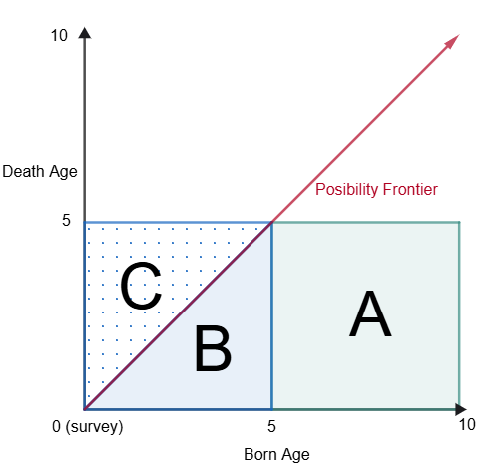
\includegraphics[width=0.4\linewidth,height=\textheight,keepaspectratio]{img/mortality_chart.png}

}

\end{figure}%

\textbf{1.2.b.i} I estimated the mortality rates for boys and girls
using both methods in R using the columns \texttt{\_l5} for method 1 and
the difference of total minus \texttt{\_l5} for method 2 (See appendix
for code). The estimated mortality rates for boys and girls using both
methods are shown in Table \ref{tbl-child_mortality}.

 
\begin{table}[ht]
\begin{centerbox}
\begin{threeparttable}
\captionsetup{justification=centering,singlelinecheck=off}
\caption{Child mortality rates in Côte d'Ivoire, by sex and method.}
 \label{tbl-child_mortality}\setlength{\tabcolsep}{0pt}
\begin{tabular}{l l l l l l l l}


\hhline{>{\huxb{0, 0, 0}{0.8}}->{\huxb{0, 0, 0}{0.8}}->{\huxb{0, 0, 0}{0.8}}->{\huxb{0, 0, 0}{0.8}}->{\huxb{0, 0, 0}{0.8}}->{\huxb{0, 0, 0}{0.8}}->{\huxb{0, 0, 0}{0.8}}->{\huxb{0, 0, 0}{0.8}}-}
\arrayrulecolor{black}

\multicolumn{1}{!{\huxvb{0, 0, 0}{0}}c!{\huxvb{0, 0, 0}{0}}}{\huxtpad{1.5pt + 1em}\centering \hspace{1.5pt}  \hspace{1.5pt}\huxbpad{1.5pt}} &
\multicolumn{1}{c!{\huxvb{0, 0, 0}{0}}}{\huxtpad{1.5pt + 1em}\centering \hspace{1.5pt} M1 (Boys) \hspace{1.5pt}\huxbpad{1.5pt}} &
\multicolumn{1}{c!{\huxvb{0, 0, 0}{0}}}{\huxtpad{1.5pt + 1em}\centering \hspace{1.5pt} M2 (Boys) \hspace{1.5pt}\huxbpad{1.5pt}} &
\multicolumn{1}{c!{\huxvb{0, 0, 0}{0}}}{\huxtpad{1.5pt + 1em}\centering \hspace{1.5pt} Diff (Boys) \hspace{1.5pt}\huxbpad{1.5pt}} &
\multicolumn{1}{c!{\huxvb{0, 0, 0}{0}}}{\huxtpad{1.5pt + 1em}\centering \hspace{1.5pt} M1 (Girls) \hspace{1.5pt}\huxbpad{1.5pt}} &
\multicolumn{1}{c!{\huxvb{0, 0, 0}{0}}}{\huxtpad{1.5pt + 1em}\centering \hspace{1.5pt} M2 (Girls) \hspace{1.5pt}\huxbpad{1.5pt}} &
\multicolumn{1}{c!{\huxvb{0, 0, 0}{0}}}{\huxtpad{1.5pt + 1em}\centering \hspace{1.5pt} Diff (Girls) \hspace{1.5pt}\huxbpad{1.5pt}} &
\multicolumn{1}{c!{\huxvb{0, 0, 0}{0}}}{\huxtpad{1.5pt + 1em}\centering \hspace{1.5pt} Diff M2 G-B \hspace{1.5pt}\huxbpad{1.5pt}} \tabularnewline[-0.5pt]


\hhline{>{\huxb{255, 255, 255}{0.4}}->{\huxb{0, 0, 0}{0.4}}->{\huxb{0, 0, 0}{0.4}}->{\huxb{0, 0, 0}{0.4}}->{\huxb{0, 0, 0}{0.4}}->{\huxb{0, 0, 0}{0.4}}->{\huxb{0, 0, 0}{0.4}}->{\huxb{0, 0, 0}{0.4}}-}
\arrayrulecolor{black}

\multicolumn{1}{!{\huxvb{0, 0, 0}{0}}l!{\huxvb{0, 0, 0}{0}}}{\huxtpad{1.5pt + 1em}\raggedright \hspace{1.5pt} Mortality rate \hspace{1.5pt}\huxbpad{1.5pt}} &
\multicolumn{1}{r!{\huxvb{0, 0, 0}{0}}}{\huxtpad{1.5pt + 1em}\raggedleft \hspace{1.5pt} 0.117 *** \hspace{1.5pt}\huxbpad{1.5pt}} &
\multicolumn{1}{r!{\huxvb{0, 0, 0}{0}}}{\huxtpad{1.5pt + 1em}\raggedleft \hspace{1.5pt} 0.135 *** \hspace{1.5pt}\huxbpad{1.5pt}} &
\multicolumn{1}{r!{\huxvb{0, 0, 0}{0}}}{\huxtpad{1.5pt + 1em}\raggedleft \hspace{1.5pt} 0.017 \hspace{1.5pt}\huxbpad{1.5pt}} &
\multicolumn{1}{r!{\huxvb{0, 0, 0}{0}}}{\huxtpad{1.5pt + 1em}\raggedleft \hspace{1.5pt} 0.084 *** \hspace{1.5pt}\huxbpad{1.5pt}} &
\multicolumn{1}{r!{\huxvb{0, 0, 0}{0}}}{\huxtpad{1.5pt + 1em}\raggedleft \hspace{1.5pt} 0.115 *** \hspace{1.5pt}\huxbpad{1.5pt}} &
\multicolumn{1}{r!{\huxvb{0, 0, 0}{0}}}{\huxtpad{1.5pt + 1em}\raggedleft \hspace{1.5pt} 0.031 *** \hspace{1.5pt}\huxbpad{1.5pt}} &
\multicolumn{1}{r!{\huxvb{0, 0, 0}{0}}}{\huxtpad{1.5pt + 1em}\raggedleft \hspace{1.5pt} -0.020 * \hspace{1.5pt}\huxbpad{1.5pt}} \tabularnewline[-0.5pt]


\hhline{}
\arrayrulecolor{black}

\multicolumn{1}{!{\huxvb{0, 0, 0}{0}}l!{\huxvb{0, 0, 0}{0}}}{\huxtpad{1.5pt + 1em}\raggedright \hspace{1.5pt}  \hspace{1.5pt}\huxbpad{1.5pt}} &
\multicolumn{1}{r!{\huxvb{0, 0, 0}{0}}}{\huxtpad{1.5pt + 1em}\raggedleft \hspace{1.5pt} (0.007) \hspace{1.5pt}\huxbpad{1.5pt}} &
\multicolumn{1}{r!{\huxvb{0, 0, 0}{0}}}{\huxtpad{1.5pt + 1em}\raggedleft \hspace{1.5pt} (0.008) \hspace{1.5pt}\huxbpad{1.5pt}} &
\multicolumn{1}{r!{\huxvb{0, 0, 0}{0}}}{\huxtpad{1.5pt + 1em}\raggedleft \hspace{1.5pt} (0.011) \hspace{1.5pt}\huxbpad{1.5pt}} &
\multicolumn{1}{r!{\huxvb{0, 0, 0}{0}}}{\huxtpad{1.5pt + 1em}\raggedleft \hspace{1.5pt} (0.007) \hspace{1.5pt}\huxbpad{1.5pt}} &
\multicolumn{1}{r!{\huxvb{0, 0, 0}{0}}}{\huxtpad{1.5pt + 1em}\raggedleft \hspace{1.5pt} (0.008) \hspace{1.5pt}\huxbpad{1.5pt}} &
\multicolumn{1}{r!{\huxvb{0, 0, 0}{0}}}{\huxtpad{1.5pt + 1em}\raggedleft \hspace{1.5pt} (0.010) \hspace{1.5pt}\huxbpad{1.5pt}} &
\multicolumn{1}{r!{\huxvb{0, 0, 0}{0}}}{\huxtpad{1.5pt + 1em}\raggedleft \hspace{1.5pt} (0.011) \hspace{1.5pt}\huxbpad{1.5pt}} \tabularnewline[-0.5pt]


\hhline{>{\huxb{255, 255, 255}{0.4}}->{\huxb{0, 0, 0}{0.4}}->{\huxb{0, 0, 0}{0.4}}->{\huxb{0, 0, 0}{0.4}}->{\huxb{0, 0, 0}{0.4}}->{\huxb{0, 0, 0}{0.4}}->{\huxb{0, 0, 0}{0.4}}->{\huxb{0, 0, 0}{0.4}}-}
\arrayrulecolor{black}

\multicolumn{1}{!{\huxvb{0, 0, 0}{0}}l!{\huxvb{0, 0, 0}{0}}}{\huxtpad{1.5pt + 1em}\raggedright \hspace{1.5pt} N \hspace{1.5pt}\huxbpad{1.5pt}} &
\multicolumn{1}{r!{\huxvb{0, 0, 0}{0}}}{\huxtpad{1.5pt + 1em}\raggedleft \hspace{1.5pt} 1431 \hspace{1.5pt}\huxbpad{1.5pt}} &
\multicolumn{1}{r!{\huxvb{0, 0, 0}{0}}}{\huxtpad{1.5pt + 1em}\raggedleft \hspace{1.5pt} 1332 \hspace{1.5pt}\huxbpad{1.5pt}} &
\multicolumn{1}{r!{\huxvb{0, 0, 0}{0}}}{\huxtpad{1.5pt + 1em}\raggedleft \hspace{1.5pt}  \hspace{1.5pt}\huxbpad{1.5pt}} &
\multicolumn{1}{r!{\huxvb{0, 0, 0}{0}}}{\huxtpad{1.5pt + 1em}\raggedleft \hspace{1.5pt} 1428 \hspace{1.5pt}\huxbpad{1.5pt}} &
\multicolumn{1}{r!{\huxvb{0, 0, 0}{0}}}{\huxtpad{1.5pt + 1em}\raggedleft \hspace{1.5pt} 1291 \hspace{1.5pt}\huxbpad{1.5pt}} &
\multicolumn{1}{r!{\huxvb{0, 0, 0}{0}}}{\huxtpad{1.5pt + 1em}\raggedleft \hspace{1.5pt}  \hspace{1.5pt}\huxbpad{1.5pt}} &
\multicolumn{1}{r!{\huxvb{0, 0, 0}{0}}}{\huxtpad{1.5pt + 1em}\raggedleft \hspace{1.5pt}  \hspace{1.5pt}\huxbpad{1.5pt}} \tabularnewline[-0.5pt]


\hhline{}
\arrayrulecolor{black}

\multicolumn{1}{!{\huxvb{0, 0, 0}{0}}l!{\huxvb{0, 0, 0}{0}}}{\huxtpad{1.5pt + 1em}\raggedright \hspace{1.5pt} R2 \hspace{1.5pt}\huxbpad{1.5pt}} &
\multicolumn{1}{r!{\huxvb{0, 0, 0}{0}}}{\huxtpad{1.5pt + 1em}\raggedleft \hspace{1.5pt} 0.000 \hspace{1.5pt}\huxbpad{1.5pt}} &
\multicolumn{1}{r!{\huxvb{0, 0, 0}{0}}}{\huxtpad{1.5pt + 1em}\raggedleft \hspace{1.5pt} 0.000 \hspace{1.5pt}\huxbpad{1.5pt}} &
\multicolumn{1}{r!{\huxvb{0, 0, 0}{0}}}{\huxtpad{1.5pt + 1em}\raggedleft \hspace{1.5pt}  \hspace{1.5pt}\huxbpad{1.5pt}} &
\multicolumn{1}{r!{\huxvb{0, 0, 0}{0}}}{\huxtpad{1.5pt + 1em}\raggedleft \hspace{1.5pt} 0.000 \hspace{1.5pt}\huxbpad{1.5pt}} &
\multicolumn{1}{r!{\huxvb{0, 0, 0}{0}}}{\huxtpad{1.5pt + 1em}\raggedleft \hspace{1.5pt} 0.000 \hspace{1.5pt}\huxbpad{1.5pt}} &
\multicolumn{1}{r!{\huxvb{0, 0, 0}{0}}}{\huxtpad{1.5pt + 1em}\raggedleft \hspace{1.5pt}  \hspace{1.5pt}\huxbpad{1.5pt}} &
\multicolumn{1}{r!{\huxvb{0, 0, 0}{0}}}{\huxtpad{1.5pt + 1em}\raggedleft \hspace{1.5pt}  \hspace{1.5pt}\huxbpad{1.5pt}} \tabularnewline[-0.5pt]


\hhline{>{\huxb{0, 0, 0}{0.8}}->{\huxb{0, 0, 0}{0.8}}->{\huxb{0, 0, 0}{0.8}}->{\huxb{0, 0, 0}{0.8}}->{\huxb{0, 0, 0}{0.8}}->{\huxb{0, 0, 0}{0.8}}->{\huxb{0, 0, 0}{0.8}}->{\huxb{0, 0, 0}{0.8}}-}
\arrayrulecolor{black}
\end{tabular}
\begin{tablenotes}[flushleft]
\item[] Significance: *** p $<$ 0.01; ** p $<$ 0.05; * p $<$ 0.1
\end{tablenotes}
\end{threeparttable}\par\end{centerbox}

\end{table}
 

\textbf{1.2.b.ii} Table \ref{tbl-child_mortality} shows the estimated
child mortality rates in Côte d'Ivoire for boys and girls using both
methods and their differences. The results confirm our theory of M1
underestimating the true mortality rate. We can clearly see the method
estimates differences are positive indicating that M1 systematically
underestimates the true mortality rate estimated by M2. Using the best
method (M2), the average mortality rate for boys is 13.5\% and for girls
is 11.9\%. The difference between girls and boys is -2 percentage points
and statistically significant at the 90\% confidence level, indicating
that boys have a higher mortality rate than girls.

\section{2 Health status, nutritional status and wealth in Côte
d'Ivoire}\label{health-status-nutritional-status-and-wealth-in-cuxf4te-divoire}

\textbf{2.1.a} Let's denote the estimated mean weight as
\(W_{\text{obs}}\), the true mean weight as \(W_{\text{true}}\), and the
proportion of weights measured in hectograms as \(p_h\). The observed
mean weight can be expressed as the sum of the mean weights measured in
kg and in hectograms multiplied by their corresponding probabilities:

\[
\begin{aligned}
E[W_{\text{obs}}] &= (1 - p_h) \cdot W_{\text{true}} + p_h \cdot W_{\text{true}}\cdot 10\\
  &= W_{\text{true}} \cdot (1 - p_h + 10 p_h)\\
  &= W_{\text{true}} \cdot (1 + 9 p_h)
\end{aligned}
\]

Thus, having an estimate of \(p_h\) would allow us to correct the
observed mean weight. Notice that if \(p_h = 0\), then
\(E[W_{\text{obs}}] = W_{\text{true}}\), and if \(p_h = 1\), then
\(E[W_{\text{obs}}] = 10 W_{\text{true}}\).

For applying the correction, it is necessary to have a good estimate of
\(p_h\). In this case, it can be approximated by the proportion of
weights above 25kg in 2008 which is 30.4\% of the observations. Using
this, we can correct the mean weight estimate by dividing the observed
mean weight by \((1 + 9 p_h)\). See Table
\ref{tbl-corrected_weight_mean} where the 2008 mean weight is corrected.
After correction, the mean weight in 2008 is \(11.48\)kg, which is
consistent with previous years.

{

\begin{longtable}[]{@{}rrrr@{}}

\caption{\label{tbl-corrected_weight_mean}Summary of Weight Estimates
With Hectogram Correction}

\tabularnewline

\toprule\noalign{}
Year & Obs & Mean Weight & Mean Weight Corrected \\
\midrule\noalign{}
\endhead
\bottomrule\noalign{}
\endlastfoot
1988 & 6475 & 12.46 & 12.46 \\
1993 & 7109 & 11.94 & 11.94 \\
2008 & 7333 & 42.87 & 11.48 \\

\end{longtable}

}

\textbf{2.1.b} By looking at the original distribution the weight
measurements in 2008 show a wider distribution than the 1988 and 1993
distributions. The 2008 distribution shows a principal component at
around 12kg but also shows multiple peaks at weight \textgreater{} 25kg
while the 1988 and 1993 distributions show a principal component at
around 12kg with minimal outliers e.g.~a few values below 1kg. See
Figure \ref{fig-distributions} LHS.

After updating the 2008 weight distribution by dividing all weights
\textgreater{} 25kg by 10, the distribution shows no peaks after 25kg.
See Figure \ref{fig-distributions} RHS.

\begin{figure}

\caption{\label{fig-distributions}Distribution of Weight (kg) Before and
After Correction}

\centering{

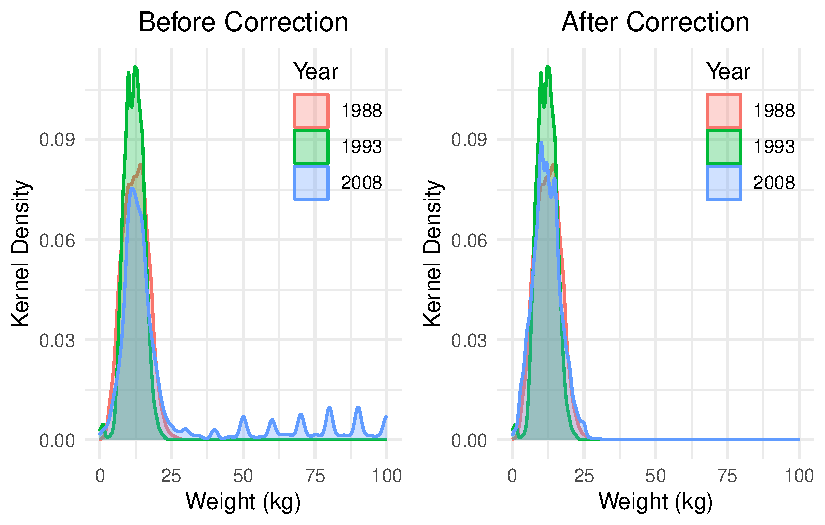
\includegraphics[width=0.7\linewidth,height=\textheight,keepaspectratio]{hw2_trimmed_files/figure-pdf/fig-distributions-1.pdf}

}

\end{figure}%

\textbf{2.2} Estimated z-scores are computed using the mentioned
formula. The resulting distribution of z-scores for 2-4 years old
children by year and region is shown in Figure
\ref{fig-distributions_stunted}.

\begin{figure}

\caption{\label{fig-distributions_stunted}Distribution of z-scores by
year}

\centering{

\subcaption{\label{fig-distributions_stunted}X-axis is limited to -6 to
6, and the dashed line indicates the stunting threshold of -2.}

\centering{

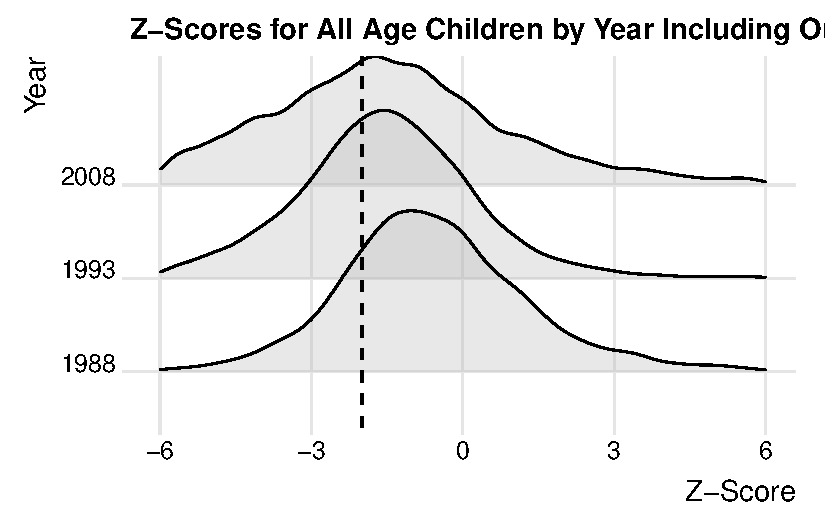
\includegraphics[width=0.7\linewidth,height=\textheight,keepaspectratio]{hw2_trimmed_files/figure-pdf/fig-distributions_stunted-1.pdf}

}

}

\end{figure}%

\textbf{2.3.a} As shown in Table \ref{tbl-stunted_north_south}, the
national stunting rate for 2-4 years old children with outliers is
24.1\% in 1988, 42\% in 1993, and 46.4\% in 2008. This increasing trend
shows an overall increment of 22.3 percentage points in the stunting
rate over the 20-year period.

The north and south regions show an increasing trend over time, but the
north region shows a higher stunting rate than the south region in 1988
and 2008. Particularly, in 1988 the difference between north and south
is 5.6 percentage points at the 1\% significance level, and in 2008 the
difference is 4.5 percentage points at the 5\% significance level. In
1993 the difference is not statistically significant different from
zero, indicating that the north and south regions had similar stunting
rates in 1993. Many theories can explain the differences between north
and south e.g.~differences in measurement, differences in the
population, or the effect of socioeconomic factors such as
poverty-alleviating programs, and access to health care.

The results excluding outliers show a similar trend in 1988 and 1993,
however, in 2008 the stunting is not as different from 1993 except in
the north region where there is a difference of 4 percentage points.
This change in the pattern suggest that the outliers correction had an
impact on the results and drafted conclusions. Regional differences
between north and south persist, there is still a significant difference
of 6.1 and 3.5 percentage points in 1988 and 2008 at the 1\% and 10\%
significance levels respectively between the north and south regions
despite the change in the stunting rate over time pattern.

 
\begin{table}[ht]
\begin{centerbox}
\begin{threeparttable}
\captionsetup{justification=centering,singlelinecheck=off}
\caption{National, North, and South stunting rates for 2-4 years old children excluding outliers.}
 \label{tbl-stunted_north_south}\setlength{\tabcolsep}{0pt}
\begin{tabularx}{1\textwidth}{p{0.111111111111111\textwidth} p{0.111111111111111\textwidth} p{0.111111111111111\textwidth} p{0.111111111111111\textwidth} p{0.111111111111111\textwidth} p{0.111111111111111\textwidth} p{0.111111111111111\textwidth} p{0.111111111111111\textwidth} p{0.111111111111111\textwidth}}


\hhline{>{\huxb{0, 0, 0}{0.8}}->{\huxb{0, 0, 0}{0.8}}->{\huxb{0, 0, 0}{0.8}}->{\huxb{0, 0, 0}{0.8}}->{\huxb{0, 0, 0}{0.8}}->{\huxb{0, 0, 0}{0.8}}->{\huxb{0, 0, 0}{0.8}}->{\huxb{0, 0, 0}{0.8}}->{\huxb{0, 0, 0}{0.8}}-}
\arrayrulecolor{black}

\multicolumn{1}{!{\huxvb{0, 0, 0}{0}}p{0.111111111111111\textwidth}!{\huxvb{0, 0, 0}{0}}}{\hspace{1.5pt}\parbox[b]{0.111111111111111\textwidth-1.5pt-1.5pt}{\huxtpad{1.5pt + 1em}\centering \huxbpad{1.5pt}}} &
\multicolumn{1}{p{0.111111111111111\textwidth}!{\huxvb{0, 0, 0}{0}}}{\hspace{1.5pt}\parbox[b]{0.111111111111111\textwidth-1.5pt-1.5pt}{\huxtpad{1.5pt + 1em}\centering National\huxbpad{1.5pt}}} &
\multicolumn{1}{p{0.111111111111111\textwidth}!{\huxvb{0, 0, 0}{0}}}{\hspace{1.5pt}\parbox[b]{0.111111111111111\textwidth-1.5pt-1.5pt}{\huxtpad{1.5pt + 1em}\centering North\huxbpad{1.5pt}}} &
\multicolumn{1}{p{0.111111111111111\textwidth}!{\huxvb{0, 0, 0}{0}}}{\hspace{1.5pt}\parbox[b]{0.111111111111111\textwidth-1.5pt-1.5pt}{\huxtpad{1.5pt + 1em}\centering South\huxbpad{1.5pt}}} &
\multicolumn{1}{p{0.111111111111111\textwidth}!{\huxvb{0, 0, 0}{0}}}{\hspace{1.5pt}\parbox[b]{0.111111111111111\textwidth-1.5pt-1.5pt}{\huxtpad{1.5pt + 1em}\centering Diff \newline (North-South)\huxbpad{1.5pt}}} &
\multicolumn{1}{p{0.111111111111111\textwidth}!{\huxvb{0, 0, 0}{0}}}{\hspace{1.5pt}\parbox[b]{0.111111111111111\textwidth-1.5pt-1.5pt}{\huxtpad{1.5pt + 1em}\centering National \huxbpad{1.5pt}}} &
\multicolumn{1}{p{0.111111111111111\textwidth}!{\huxvb{0, 0, 0}{0}}}{\hspace{1.5pt}\parbox[b]{0.111111111111111\textwidth-1.5pt-1.5pt}{\huxtpad{1.5pt + 1em}\centering North \huxbpad{1.5pt}}} &
\multicolumn{1}{p{0.111111111111111\textwidth}!{\huxvb{0, 0, 0}{0}}}{\hspace{1.5pt}\parbox[b]{0.111111111111111\textwidth-1.5pt-1.5pt}{\huxtpad{1.5pt + 1em}\centering South \huxbpad{1.5pt}}} &
\multicolumn{1}{p{0.111111111111111\textwidth}!{\huxvb{0, 0, 0}{0}}}{\hspace{1.5pt}\parbox[b]{0.111111111111111\textwidth-1.5pt-1.5pt}{\huxtpad{1.5pt + 1em}\centering Diff \newline (North-South) \huxbpad{1.5pt}}} \tabularnewline[-0.5pt]


\hhline{>{\huxb{255, 255, 255}{0.4}}->{\huxb{0, 0, 0}{0.4}}->{\huxb{0, 0, 0}{0.4}}->{\huxb{0, 0, 0}{0.4}}->{\huxb{0, 0, 0}{0.4}}->{\huxb{0, 0, 0}{0.4}}->{\huxb{0, 0, 0}{0.4}}->{\huxb{0, 0, 0}{0.4}}->{\huxb{0, 0, 0}{0.4}}-}
\arrayrulecolor{black}

\multicolumn{1}{!{\huxvb{0, 0, 0}{0}}p{0.111111111111111\textwidth}!{\huxvb{0, 0, 0}{0}}}{\hspace{1.5pt}\parbox[b]{0.111111111111111\textwidth-1.5pt-1.5pt}{\huxtpad{1.5pt + 1em}\raggedright Year 1988\huxbpad{1.5pt}}} &
\multicolumn{1}{p{0.111111111111111\textwidth}!{\huxvb{0, 0, 0}{0}}}{\hspace{1.5pt}\parbox[b]{0.111111111111111\textwidth-1.5pt-1.5pt}{\huxtpad{1.5pt + 1em}\raggedleft 0.241 ***\huxbpad{1.5pt}}} &
\multicolumn{1}{p{0.111111111111111\textwidth}!{\huxvb{0, 0, 0}{0}}}{\hspace{1.5pt}\parbox[b]{0.111111111111111\textwidth-1.5pt-1.5pt}{\huxtpad{1.5pt + 1em}\raggedleft 0.282 ***\huxbpad{1.5pt}}} &
\multicolumn{1}{p{0.111111111111111\textwidth}!{\huxvb{0, 0, 0}{0}}}{\hspace{1.5pt}\parbox[b]{0.111111111111111\textwidth-1.5pt-1.5pt}{\huxtpad{1.5pt + 1em}\raggedleft 0.226 ***\huxbpad{1.5pt}}} &
\multicolumn{1}{p{0.111111111111111\textwidth}!{\huxvb{0, 0, 0}{0}}}{\hspace{1.5pt}\parbox[b]{0.111111111111111\textwidth-1.5pt-1.5pt}{\huxtpad{1.5pt + 1em}\raggedleft 0.056 ***\huxbpad{1.5pt}}} &
\multicolumn{1}{p{0.111111111111111\textwidth}!{\huxvb{0, 0, 0}{0}}}{\hspace{1.5pt}\parbox[b]{0.111111111111111\textwidth-1.5pt-1.5pt}{\huxtpad{1.5pt + 1em}\raggedleft 0.239 ***\huxbpad{1.5pt}}} &
\multicolumn{1}{p{0.111111111111111\textwidth}!{\huxvb{0, 0, 0}{0}}}{\hspace{1.5pt}\parbox[b]{0.111111111111111\textwidth-1.5pt-1.5pt}{\huxtpad{1.5pt + 1em}\raggedleft 0.284 ***\huxbpad{1.5pt}}} &
\multicolumn{1}{p{0.111111111111111\textwidth}!{\huxvb{0, 0, 0}{0}}}{\hspace{1.5pt}\parbox[b]{0.111111111111111\textwidth-1.5pt-1.5pt}{\huxtpad{1.5pt + 1em}\raggedleft 0.222 ***\huxbpad{1.5pt}}} &
\multicolumn{1}{p{0.111111111111111\textwidth}!{\huxvb{0, 0, 0}{0}}}{\hspace{1.5pt}\parbox[b]{0.111111111111111\textwidth-1.5pt-1.5pt}{\huxtpad{1.5pt + 1em}\raggedleft 0.061 ***\huxbpad{1.5pt}}} \tabularnewline[-0.5pt]


\hhline{}
\arrayrulecolor{black}

\multicolumn{1}{!{\huxvb{0, 0, 0}{0}}p{0.111111111111111\textwidth}!{\huxvb{0, 0, 0}{0}}}{\hspace{1.5pt}\parbox[b]{0.111111111111111\textwidth-1.5pt-1.5pt}{\huxtpad{1.5pt + 1em}\raggedright \huxbpad{1.5pt}}} &
\multicolumn{1}{p{0.111111111111111\textwidth}!{\huxvb{0, 0, 0}{0}}}{\hspace{1.5pt}\parbox[b]{0.111111111111111\textwidth-1.5pt-1.5pt}{\huxtpad{1.5pt + 1em}\raggedleft (0.009)\huxbpad{1.5pt}}} &
\multicolumn{1}{p{0.111111111111111\textwidth}!{\huxvb{0, 0, 0}{0}}}{\hspace{1.5pt}\parbox[b]{0.111111111111111\textwidth-1.5pt-1.5pt}{\huxtpad{1.5pt + 1em}\raggedleft (0.016)\huxbpad{1.5pt}}} &
\multicolumn{1}{p{0.111111111111111\textwidth}!{\huxvb{0, 0, 0}{0}}}{\hspace{1.5pt}\parbox[b]{0.111111111111111\textwidth-1.5pt-1.5pt}{\huxtpad{1.5pt + 1em}\raggedleft (0.011)\huxbpad{1.5pt}}} &
\multicolumn{1}{p{0.111111111111111\textwidth}!{\huxvb{0, 0, 0}{0}}}{\hspace{1.5pt}\parbox[b]{0.111111111111111\textwidth-1.5pt-1.5pt}{\huxtpad{1.5pt + 1em}\raggedleft (0.020)\huxbpad{1.5pt}}} &
\multicolumn{1}{p{0.111111111111111\textwidth}!{\huxvb{0, 0, 0}{0}}}{\hspace{1.5pt}\parbox[b]{0.111111111111111\textwidth-1.5pt-1.5pt}{\huxtpad{1.5pt + 1em}\raggedleft (0.009)\huxbpad{1.5pt}}} &
\multicolumn{1}{p{0.111111111111111\textwidth}!{\huxvb{0, 0, 0}{0}}}{\hspace{1.5pt}\parbox[b]{0.111111111111111\textwidth-1.5pt-1.5pt}{\huxtpad{1.5pt + 1em}\raggedleft (0.016)\huxbpad{1.5pt}}} &
\multicolumn{1}{p{0.111111111111111\textwidth}!{\huxvb{0, 0, 0}{0}}}{\hspace{1.5pt}\parbox[b]{0.111111111111111\textwidth-1.5pt-1.5pt}{\huxtpad{1.5pt + 1em}\raggedleft (0.010)\huxbpad{1.5pt}}} &
\multicolumn{1}{p{0.111111111111111\textwidth}!{\huxvb{0, 0, 0}{0}}}{\hspace{1.5pt}\parbox[b]{0.111111111111111\textwidth-1.5pt-1.5pt}{\huxtpad{1.5pt + 1em}\raggedleft (0.020)\huxbpad{1.5pt}}} \tabularnewline[-0.5pt]


\hhline{}
\arrayrulecolor{black}

\multicolumn{1}{!{\huxvb{0, 0, 0}{0}}p{0.111111111111111\textwidth}!{\huxvb{0, 0, 0}{0}}}{\hspace{1.5pt}\parbox[b]{0.111111111111111\textwidth-1.5pt-1.5pt}{\huxtpad{1.5pt + 1em}\raggedright Year 1993\huxbpad{1.5pt}}} &
\multicolumn{1}{p{0.111111111111111\textwidth}!{\huxvb{0, 0, 0}{0}}}{\hspace{1.5pt}\parbox[b]{0.111111111111111\textwidth-1.5pt-1.5pt}{\huxtpad{1.5pt + 1em}\raggedleft 0.420 ***\huxbpad{1.5pt}}} &
\multicolumn{1}{p{0.111111111111111\textwidth}!{\huxvb{0, 0, 0}{0}}}{\hspace{1.5pt}\parbox[b]{0.111111111111111\textwidth-1.5pt-1.5pt}{\huxtpad{1.5pt + 1em}\raggedleft 0.409 ***\huxbpad{1.5pt}}} &
\multicolumn{1}{p{0.111111111111111\textwidth}!{\huxvb{0, 0, 0}{0}}}{\hspace{1.5pt}\parbox[b]{0.111111111111111\textwidth-1.5pt-1.5pt}{\huxtpad{1.5pt + 1em}\raggedleft 0.423 ***\huxbpad{1.5pt}}} &
\multicolumn{1}{p{0.111111111111111\textwidth}!{\huxvb{0, 0, 0}{0}}}{\hspace{1.5pt}\parbox[b]{0.111111111111111\textwidth-1.5pt-1.5pt}{\huxtpad{1.5pt + 1em}\raggedleft -0.014\huxbpad{1.5pt}}} &
\multicolumn{1}{p{0.111111111111111\textwidth}!{\huxvb{0, 0, 0}{0}}}{\hspace{1.5pt}\parbox[b]{0.111111111111111\textwidth-1.5pt-1.5pt}{\huxtpad{1.5pt + 1em}\raggedleft 0.412 ***\huxbpad{1.5pt}}} &
\multicolumn{1}{p{0.111111111111111\textwidth}!{\huxvb{0, 0, 0}{0}}}{\hspace{1.5pt}\parbox[b]{0.111111111111111\textwidth-1.5pt-1.5pt}{\huxtpad{1.5pt + 1em}\raggedleft 0.397 ***\huxbpad{1.5pt}}} &
\multicolumn{1}{p{0.111111111111111\textwidth}!{\huxvb{0, 0, 0}{0}}}{\hspace{1.5pt}\parbox[b]{0.111111111111111\textwidth-1.5pt-1.5pt}{\huxtpad{1.5pt + 1em}\raggedleft 0.416 ***\huxbpad{1.5pt}}} &
\multicolumn{1}{p{0.111111111111111\textwidth}!{\huxvb{0, 0, 0}{0}}}{\hspace{1.5pt}\parbox[b]{0.111111111111111\textwidth-1.5pt-1.5pt}{\huxtpad{1.5pt + 1em}\raggedleft -0.020\huxbpad{1.5pt}}} \tabularnewline[-0.5pt]


\hhline{}
\arrayrulecolor{black}

\multicolumn{1}{!{\huxvb{0, 0, 0}{0}}p{0.111111111111111\textwidth}!{\huxvb{0, 0, 0}{0}}}{\hspace{1.5pt}\parbox[b]{0.111111111111111\textwidth-1.5pt-1.5pt}{\huxtpad{1.5pt + 1em}\raggedright \huxbpad{1.5pt}}} &
\multicolumn{1}{p{0.111111111111111\textwidth}!{\huxvb{0, 0, 0}{0}}}{\hspace{1.5pt}\parbox[b]{0.111111111111111\textwidth-1.5pt-1.5pt}{\huxtpad{1.5pt + 1em}\raggedleft (0.007)\huxbpad{1.5pt}}} &
\multicolumn{1}{p{0.111111111111111\textwidth}!{\huxvb{0, 0, 0}{0}}}{\hspace{1.5pt}\parbox[b]{0.111111111111111\textwidth-1.5pt-1.5pt}{\huxtpad{1.5pt + 1em}\raggedleft (0.014)\huxbpad{1.5pt}}} &
\multicolumn{1}{p{0.111111111111111\textwidth}!{\huxvb{0, 0, 0}{0}}}{\hspace{1.5pt}\parbox[b]{0.111111111111111\textwidth-1.5pt-1.5pt}{\huxtpad{1.5pt + 1em}\raggedleft (0.008)\huxbpad{1.5pt}}} &
\multicolumn{1}{p{0.111111111111111\textwidth}!{\huxvb{0, 0, 0}{0}}}{\hspace{1.5pt}\parbox[b]{0.111111111111111\textwidth-1.5pt-1.5pt}{\huxtpad{1.5pt + 1em}\raggedleft (0.017)\huxbpad{1.5pt}}} &
\multicolumn{1}{p{0.111111111111111\textwidth}!{\huxvb{0, 0, 0}{0}}}{\hspace{1.5pt}\parbox[b]{0.111111111111111\textwidth-1.5pt-1.5pt}{\huxtpad{1.5pt + 1em}\raggedleft (0.007)\huxbpad{1.5pt}}} &
\multicolumn{1}{p{0.111111111111111\textwidth}!{\huxvb{0, 0, 0}{0}}}{\hspace{1.5pt}\parbox[b]{0.111111111111111\textwidth-1.5pt-1.5pt}{\huxtpad{1.5pt + 1em}\raggedleft (0.014)\huxbpad{1.5pt}}} &
\multicolumn{1}{p{0.111111111111111\textwidth}!{\huxvb{0, 0, 0}{0}}}{\hspace{1.5pt}\parbox[b]{0.111111111111111\textwidth-1.5pt-1.5pt}{\huxtpad{1.5pt + 1em}\raggedleft (0.008)\huxbpad{1.5pt}}} &
\multicolumn{1}{p{0.111111111111111\textwidth}!{\huxvb{0, 0, 0}{0}}}{\hspace{1.5pt}\parbox[b]{0.111111111111111\textwidth-1.5pt-1.5pt}{\huxtpad{1.5pt + 1em}\raggedleft (0.017)\huxbpad{1.5pt}}} \tabularnewline[-0.5pt]


\hhline{}
\arrayrulecolor{black}

\multicolumn{1}{!{\huxvb{0, 0, 0}{0}}p{0.111111111111111\textwidth}!{\huxvb{0, 0, 0}{0}}}{\hspace{1.5pt}\parbox[b]{0.111111111111111\textwidth-1.5pt-1.5pt}{\huxtpad{1.5pt + 1em}\raggedright Year 2008\huxbpad{1.5pt}}} &
\multicolumn{1}{p{0.111111111111111\textwidth}!{\huxvb{0, 0, 0}{0}}}{\hspace{1.5pt}\parbox[b]{0.111111111111111\textwidth-1.5pt-1.5pt}{\huxtpad{1.5pt + 1em}\raggedleft 0.464 ***\huxbpad{1.5pt}}} &
\multicolumn{1}{p{0.111111111111111\textwidth}!{\huxvb{0, 0, 0}{0}}}{\hspace{1.5pt}\parbox[b]{0.111111111111111\textwidth-1.5pt-1.5pt}{\huxtpad{1.5pt + 1em}\raggedleft 0.498 ***\huxbpad{1.5pt}}} &
\multicolumn{1}{p{0.111111111111111\textwidth}!{\huxvb{0, 0, 0}{0}}}{\hspace{1.5pt}\parbox[b]{0.111111111111111\textwidth-1.5pt-1.5pt}{\huxtpad{1.5pt + 1em}\raggedleft 0.453 ***\huxbpad{1.5pt}}} &
\multicolumn{1}{p{0.111111111111111\textwidth}!{\huxvb{0, 0, 0}{0}}}{\hspace{1.5pt}\parbox[b]{0.111111111111111\textwidth-1.5pt-1.5pt}{\huxtpad{1.5pt + 1em}\raggedleft 0.045 **\huxbpad{1.5pt}}} &
\multicolumn{1}{p{0.111111111111111\textwidth}!{\huxvb{0, 0, 0}{0}}}{\hspace{1.5pt}\parbox[b]{0.111111111111111\textwidth-1.5pt-1.5pt}{\huxtpad{1.5pt + 1em}\raggedleft 0.410 ***\huxbpad{1.5pt}}} &
\multicolumn{1}{p{0.111111111111111\textwidth}!{\huxvb{0, 0, 0}{0}}}{\hspace{1.5pt}\parbox[b]{0.111111111111111\textwidth-1.5pt-1.5pt}{\huxtpad{1.5pt + 1em}\raggedleft 0.436 ***\huxbpad{1.5pt}}} &
\multicolumn{1}{p{0.111111111111111\textwidth}!{\huxvb{0, 0, 0}{0}}}{\hspace{1.5pt}\parbox[b]{0.111111111111111\textwidth-1.5pt-1.5pt}{\huxtpad{1.5pt + 1em}\raggedleft 0.402 ***\huxbpad{1.5pt}}} &
\multicolumn{1}{p{0.111111111111111\textwidth}!{\huxvb{0, 0, 0}{0}}}{\hspace{1.5pt}\parbox[b]{0.111111111111111\textwidth-1.5pt-1.5pt}{\huxtpad{1.5pt + 1em}\raggedleft 0.035 *\huxbpad{1.5pt}}} \tabularnewline[-0.5pt]


\hhline{}
\arrayrulecolor{black}

\multicolumn{1}{!{\huxvb{0, 0, 0}{0}}p{0.111111111111111\textwidth}!{\huxvb{0, 0, 0}{0}}}{\hspace{1.5pt}\parbox[b]{0.111111111111111\textwidth-1.5pt-1.5pt}{\huxtpad{1.5pt + 1em}\raggedright \huxbpad{1.5pt}}} &
\multicolumn{1}{p{0.111111111111111\textwidth}!{\huxvb{0, 0, 0}{0}}}{\hspace{1.5pt}\parbox[b]{0.111111111111111\textwidth-1.5pt-1.5pt}{\huxtpad{1.5pt + 1em}\raggedleft (0.008)\huxbpad{1.5pt}}} &
\multicolumn{1}{p{0.111111111111111\textwidth}!{\huxvb{0, 0, 0}{0}}}{\hspace{1.5pt}\parbox[b]{0.111111111111111\textwidth-1.5pt-1.5pt}{\huxtpad{1.5pt + 1em}\raggedleft (0.015)\huxbpad{1.5pt}}} &
\multicolumn{1}{p{0.111111111111111\textwidth}!{\huxvb{0, 0, 0}{0}}}{\hspace{1.5pt}\parbox[b]{0.111111111111111\textwidth-1.5pt-1.5pt}{\huxtpad{1.5pt + 1em}\raggedleft (0.009)\huxbpad{1.5pt}}} &
\multicolumn{1}{p{0.111111111111111\textwidth}!{\huxvb{0, 0, 0}{0}}}{\hspace{1.5pt}\parbox[b]{0.111111111111111\textwidth-1.5pt-1.5pt}{\huxtpad{1.5pt + 1em}\raggedleft (0.018)\huxbpad{1.5pt}}} &
\multicolumn{1}{p{0.111111111111111\textwidth}!{\huxvb{0, 0, 0}{0}}}{\hspace{1.5pt}\parbox[b]{0.111111111111111\textwidth-1.5pt-1.5pt}{\huxtpad{1.5pt + 1em}\raggedleft (0.008)\huxbpad{1.5pt}}} &
\multicolumn{1}{p{0.111111111111111\textwidth}!{\huxvb{0, 0, 0}{0}}}{\hspace{1.5pt}\parbox[b]{0.111111111111111\textwidth-1.5pt-1.5pt}{\huxtpad{1.5pt + 1em}\raggedleft (0.016)\huxbpad{1.5pt}}} &
\multicolumn{1}{p{0.111111111111111\textwidth}!{\huxvb{0, 0, 0}{0}}}{\hspace{1.5pt}\parbox[b]{0.111111111111111\textwidth-1.5pt-1.5pt}{\huxtpad{1.5pt + 1em}\raggedleft (0.010)\huxbpad{1.5pt}}} &
\multicolumn{1}{p{0.111111111111111\textwidth}!{\huxvb{0, 0, 0}{0}}}{\hspace{1.5pt}\parbox[b]{0.111111111111111\textwidth-1.5pt-1.5pt}{\huxtpad{1.5pt + 1em}\raggedleft (0.019)\huxbpad{1.5pt}}} \tabularnewline[-0.5pt]


\hhline{>{\huxb{255, 255, 255}{0.4}}->{\huxb{0, 0, 0}{0.4}}->{\huxb{0, 0, 0}{0.4}}->{\huxb{0, 0, 0}{0.4}}->{\huxb{0, 0, 0}{0.4}}->{\huxb{0, 0, 0}{0.4}}->{\huxb{0, 0, 0}{0.4}}->{\huxb{0, 0, 0}{0.4}}->{\huxb{0, 0, 0}{0.4}}-}
\arrayrulecolor{black}

\multicolumn{1}{!{\huxvb{0, 0, 0}{0}}p{0.111111111111111\textwidth}!{\huxvb{0, 0, 0}{0}}}{\hspace{1.5pt}\parbox[b]{0.111111111111111\textwidth-1.5pt-1.5pt}{\huxtpad{1.5pt + 1em}\raggedright Outliers\huxbpad{1.5pt}}} &
\multicolumn{1}{p{0.111111111111111\textwidth}!{\huxvb{0, 0, 0}{0}}}{\hspace{1.5pt}\parbox[b]{0.111111111111111\textwidth-1.5pt-1.5pt}{\huxtpad{1.5pt + 1em}\centering Yes\huxbpad{1.5pt}}} &
\multicolumn{1}{p{0.111111111111111\textwidth}!{\huxvb{0, 0, 0}{0}}}{\hspace{1.5pt}\parbox[b]{0.111111111111111\textwidth-1.5pt-1.5pt}{\huxtpad{1.5pt + 1em}\centering Yes\huxbpad{1.5pt}}} &
\multicolumn{1}{p{0.111111111111111\textwidth}!{\huxvb{0, 0, 0}{0}}}{\hspace{1.5pt}\parbox[b]{0.111111111111111\textwidth-1.5pt-1.5pt}{\huxtpad{1.5pt + 1em}\centering Yes\huxbpad{1.5pt}}} &
\multicolumn{1}{p{0.111111111111111\textwidth}!{\huxvb{0, 0, 0}{0}}}{\hspace{1.5pt}\parbox[b]{0.111111111111111\textwidth-1.5pt-1.5pt}{\huxtpad{1.5pt + 1em}\centering Yes\huxbpad{1.5pt}}} &
\multicolumn{1}{p{0.111111111111111\textwidth}!{\huxvb{0, 0, 0}{0}}}{\hspace{1.5pt}\parbox[b]{0.111111111111111\textwidth-1.5pt-1.5pt}{\huxtpad{1.5pt + 1em}\centering No\huxbpad{1.5pt}}} &
\multicolumn{1}{p{0.111111111111111\textwidth}!{\huxvb{0, 0, 0}{0}}}{\hspace{1.5pt}\parbox[b]{0.111111111111111\textwidth-1.5pt-1.5pt}{\huxtpad{1.5pt + 1em}\centering No\huxbpad{1.5pt}}} &
\multicolumn{1}{p{0.111111111111111\textwidth}!{\huxvb{0, 0, 0}{0}}}{\hspace{1.5pt}\parbox[b]{0.111111111111111\textwidth-1.5pt-1.5pt}{\huxtpad{1.5pt + 1em}\centering No\huxbpad{1.5pt}}} &
\multicolumn{1}{p{0.111111111111111\textwidth}!{\huxvb{0, 0, 0}{0}}}{\hspace{1.5pt}\parbox[b]{0.111111111111111\textwidth-1.5pt-1.5pt}{\huxtpad{1.5pt + 1em}\centering No\huxbpad{1.5pt}}} \tabularnewline[-0.5pt]


\hhline{>{\huxb{255, 255, 255}{0.4}}->{\huxb{0, 0, 0}{0.4}}->{\huxb{0, 0, 0}{0.4}}->{\huxb{0, 0, 0}{0.4}}->{\huxb{0, 0, 0}{0.4}}->{\huxb{0, 0, 0}{0.4}}->{\huxb{0, 0, 0}{0.4}}->{\huxb{0, 0, 0}{0.4}}->{\huxb{0, 0, 0}{0.4}}-}
\arrayrulecolor{black}

\multicolumn{1}{!{\huxvb{0, 0, 0}{0}}p{0.111111111111111\textwidth}!{\huxvb{0, 0, 0}{0}}}{\hspace{1.5pt}\parbox[b]{0.111111111111111\textwidth-1.5pt-1.5pt}{\huxtpad{1.5pt + 1em}\raggedright N\huxbpad{1.5pt}}} &
\multicolumn{1}{p{0.111111111111111\textwidth}!{\huxvb{0, 0, 0}{0}}}{\hspace{1.5pt}\parbox[b]{0.111111111111111\textwidth-1.5pt-1.5pt}{\huxtpad{1.5pt + 1em}\raggedleft 11755\huxbpad{1.5pt}}} &
\multicolumn{1}{p{0.111111111111111\textwidth}!{\huxvb{0, 0, 0}{0}}}{\hspace{1.5pt}\parbox[b]{0.111111111111111\textwidth-1.5pt-1.5pt}{\huxtpad{1.5pt + 1em}\raggedleft 3194\huxbpad{1.5pt}}} &
\multicolumn{1}{p{0.111111111111111\textwidth}!{\huxvb{0, 0, 0}{0}}}{\hspace{1.5pt}\parbox[b]{0.111111111111111\textwidth-1.5pt-1.5pt}{\huxtpad{1.5pt + 1em}\raggedleft 8561\huxbpad{1.5pt}}} &
\multicolumn{1}{p{0.111111111111111\textwidth}!{\huxvb{0, 0, 0}{0}}}{\hspace{1.5pt}\parbox[b]{0.111111111111111\textwidth-1.5pt-1.5pt}{\huxtpad{1.5pt + 1em}\raggedleft \huxbpad{1.5pt}}} &
\multicolumn{1}{p{0.111111111111111\textwidth}!{\huxvb{0, 0, 0}{0}}}{\hspace{1.5pt}\parbox[b]{0.111111111111111\textwidth-1.5pt-1.5pt}{\huxtpad{1.5pt + 1em}\raggedleft 10897\huxbpad{1.5pt}}} &
\multicolumn{1}{p{0.111111111111111\textwidth}!{\huxvb{0, 0, 0}{0}}}{\hspace{1.5pt}\parbox[b]{0.111111111111111\textwidth-1.5pt-1.5pt}{\huxtpad{1.5pt + 1em}\raggedleft 2930\huxbpad{1.5pt}}} &
\multicolumn{1}{p{0.111111111111111\textwidth}!{\huxvb{0, 0, 0}{0}}}{\hspace{1.5pt}\parbox[b]{0.111111111111111\textwidth-1.5pt-1.5pt}{\huxtpad{1.5pt + 1em}\raggedleft 7967\huxbpad{1.5pt}}} &
\multicolumn{1}{p{0.111111111111111\textwidth}!{\huxvb{0, 0, 0}{0}}}{\hspace{1.5pt}\parbox[b]{0.111111111111111\textwidth-1.5pt-1.5pt}{\huxtpad{1.5pt + 1em}\raggedleft \huxbpad{1.5pt}}} \tabularnewline[-0.5pt]


\hhline{}
\arrayrulecolor{black}

\multicolumn{1}{!{\huxvb{0, 0, 0}{0}}p{0.111111111111111\textwidth}!{\huxvb{0, 0, 0}{0}}}{\hspace{1.5pt}\parbox[b]{0.111111111111111\textwidth-1.5pt-1.5pt}{\huxtpad{1.5pt + 1em}\raggedright R2\huxbpad{1.5pt}}} &
\multicolumn{1}{p{0.111111111111111\textwidth}!{\huxvb{0, 0, 0}{0}}}{\hspace{1.5pt}\parbox[b]{0.111111111111111\textwidth-1.5pt-1.5pt}{\huxtpad{1.5pt + 1em}\raggedleft 0.410\huxbpad{1.5pt}}} &
\multicolumn{1}{p{0.111111111111111\textwidth}!{\huxvb{0, 0, 0}{0}}}{\hspace{1.5pt}\parbox[b]{0.111111111111111\textwidth-1.5pt-1.5pt}{\huxtpad{1.5pt + 1em}\raggedleft 0.421\huxbpad{1.5pt}}} &
\multicolumn{1}{p{0.111111111111111\textwidth}!{\huxvb{0, 0, 0}{0}}}{\hspace{1.5pt}\parbox[b]{0.111111111111111\textwidth-1.5pt-1.5pt}{\huxtpad{1.5pt + 1em}\raggedleft 0.407\huxbpad{1.5pt}}} &
\multicolumn{1}{p{0.111111111111111\textwidth}!{\huxvb{0, 0, 0}{0}}}{\hspace{1.5pt}\parbox[b]{0.111111111111111\textwidth-1.5pt-1.5pt}{\huxtpad{1.5pt + 1em}\raggedleft \huxbpad{1.5pt}}} &
\multicolumn{1}{p{0.111111111111111\textwidth}!{\huxvb{0, 0, 0}{0}}}{\hspace{1.5pt}\parbox[b]{0.111111111111111\textwidth-1.5pt-1.5pt}{\huxtpad{1.5pt + 1em}\raggedleft 0.381\huxbpad{1.5pt}}} &
\multicolumn{1}{p{0.111111111111111\textwidth}!{\huxvb{0, 0, 0}{0}}}{\hspace{1.5pt}\parbox[b]{0.111111111111111\textwidth-1.5pt-1.5pt}{\huxtpad{1.5pt + 1em}\raggedleft 0.384\huxbpad{1.5pt}}} &
\multicolumn{1}{p{0.111111111111111\textwidth}!{\huxvb{0, 0, 0}{0}}}{\hspace{1.5pt}\parbox[b]{0.111111111111111\textwidth-1.5pt-1.5pt}{\huxtpad{1.5pt + 1em}\raggedleft 0.381\huxbpad{1.5pt}}} &
\multicolumn{1}{p{0.111111111111111\textwidth}!{\huxvb{0, 0, 0}{0}}}{\hspace{1.5pt}\parbox[b]{0.111111111111111\textwidth-1.5pt-1.5pt}{\huxtpad{1.5pt + 1em}\raggedleft \huxbpad{1.5pt}}} \tabularnewline[-0.5pt]


\hhline{>{\huxb{0, 0, 0}{0.8}}->{\huxb{0, 0, 0}{0.8}}->{\huxb{0, 0, 0}{0.8}}->{\huxb{0, 0, 0}{0.8}}->{\huxb{0, 0, 0}{0.8}}->{\huxb{0, 0, 0}{0.8}}->{\huxb{0, 0, 0}{0.8}}->{\huxb{0, 0, 0}{0.8}}->{\huxb{0, 0, 0}{0.8}}-}
\arrayrulecolor{black}
\end{tabularx}
\begin{tablenotes}[flushleft]
\item[] Significance: *** p $<$ 0.01; ** p $<$ 0.05; * p $<$ 0.1
\end{tablenotes}
\end{threeparttable}\par\end{centerbox}

\end{table}
 

\textbf{2.3.b} As shown in Table \ref{tbl-stunted_sexe}, the stunting
rate for boys and girls is increasing over time for the model with
outliers (LHS four models). Starting from 1988, boys and girls had a
stunting rate of 24.6\% and 23.6\% with no significant difference. In
1993, boys and girls had a stunting rate of 43\% and 40\% with a
significant difference of 3 percentage points indicating boys had a
higher stunting rate. In 2008, boys and girls had a stunting rate of
47\% and 45\% respectively with no significant difference.

The stunting rates pattern without outliers (RHS four columns) changes
in 2008. In this period, removing the outliers lowered the national
stunting rates from 47\% with outliers to 41\% without outliers.
Differences between boys and girls are significant at 5\% significance
level in 1993, while there is no significant difference in 1988 and
2008.

 
\begin{table}[ht]
\begin{centerbox}
\begin{threeparttable}
\captionsetup{justification=centering,singlelinecheck=off}
\caption{National, Male, and Female stunting rates for 2-4 years old children.}
 \label{tbl-stunted_sexe}\setlength{\tabcolsep}{0pt}
\begin{tabularx}{1\textwidth}{p{0.111111111111111\textwidth} p{0.111111111111111\textwidth} p{0.111111111111111\textwidth} p{0.111111111111111\textwidth} p{0.111111111111111\textwidth} p{0.111111111111111\textwidth} p{0.111111111111111\textwidth} p{0.111111111111111\textwidth} p{0.111111111111111\textwidth}}


\hhline{>{\huxb{0, 0, 0}{0.8}}->{\huxb{0, 0, 0}{0.8}}->{\huxb{0, 0, 0}{0.8}}->{\huxb{0, 0, 0}{0.8}}->{\huxb{0, 0, 0}{0.8}}->{\huxb{0, 0, 0}{0.8}}->{\huxb{0, 0, 0}{0.8}}->{\huxb{0, 0, 0}{0.8}}->{\huxb{0, 0, 0}{0.8}}-}
\arrayrulecolor{black}

\multicolumn{1}{!{\huxvb{0, 0, 0}{0}}p{0.111111111111111\textwidth}!{\huxvb{0, 0, 0}{0}}}{\hspace{1.5pt}\parbox[b]{0.111111111111111\textwidth-1.5pt-1.5pt}{\huxtpad{1.5pt + 1em}\centering \huxbpad{1.5pt}}} &
\multicolumn{1}{p{0.111111111111111\textwidth}!{\huxvb{0, 0, 0}{0}}}{\hspace{1.5pt}\parbox[b]{0.111111111111111\textwidth-1.5pt-1.5pt}{\huxtpad{1.5pt + 1em}\centering National\huxbpad{1.5pt}}} &
\multicolumn{1}{p{0.111111111111111\textwidth}!{\huxvb{0, 0, 0}{0}}}{\hspace{1.5pt}\parbox[b]{0.111111111111111\textwidth-1.5pt-1.5pt}{\huxtpad{1.5pt + 1em}\centering Male\huxbpad{1.5pt}}} &
\multicolumn{1}{p{0.111111111111111\textwidth}!{\huxvb{0, 0, 0}{0}}}{\hspace{1.5pt}\parbox[b]{0.111111111111111\textwidth-1.5pt-1.5pt}{\huxtpad{1.5pt + 1em}\centering Female\huxbpad{1.5pt}}} &
\multicolumn{1}{p{0.111111111111111\textwidth}!{\huxvb{0, 0, 0}{0}}}{\hspace{1.5pt}\parbox[b]{0.111111111111111\textwidth-1.5pt-1.5pt}{\huxtpad{1.5pt + 1em}\centering Diff \newline (Male-Female)\huxbpad{1.5pt}}} &
\multicolumn{1}{p{0.111111111111111\textwidth}!{\huxvb{0, 0, 0}{0}}}{\hspace{1.5pt}\parbox[b]{0.111111111111111\textwidth-1.5pt-1.5pt}{\huxtpad{1.5pt + 1em}\centering National \huxbpad{1.5pt}}} &
\multicolumn{1}{p{0.111111111111111\textwidth}!{\huxvb{0, 0, 0}{0}}}{\hspace{1.5pt}\parbox[b]{0.111111111111111\textwidth-1.5pt-1.5pt}{\huxtpad{1.5pt + 1em}\centering Male \huxbpad{1.5pt}}} &
\multicolumn{1}{p{0.111111111111111\textwidth}!{\huxvb{0, 0, 0}{0}}}{\hspace{1.5pt}\parbox[b]{0.111111111111111\textwidth-1.5pt-1.5pt}{\huxtpad{1.5pt + 1em}\centering Female \huxbpad{1.5pt}}} &
\multicolumn{1}{p{0.111111111111111\textwidth}!{\huxvb{0, 0, 0}{0}}}{\hspace{1.5pt}\parbox[b]{0.111111111111111\textwidth-1.5pt-1.5pt}{\huxtpad{1.5pt + 1em}\centering Diff \newline (Male-Female) \huxbpad{1.5pt}}} \tabularnewline[-0.5pt]


\hhline{>{\huxb{255, 255, 255}{0.4}}->{\huxb{0, 0, 0}{0.4}}->{\huxb{0, 0, 0}{0.4}}->{\huxb{0, 0, 0}{0.4}}->{\huxb{0, 0, 0}{0.4}}->{\huxb{0, 0, 0}{0.4}}->{\huxb{0, 0, 0}{0.4}}->{\huxb{0, 0, 0}{0.4}}->{\huxb{0, 0, 0}{0.4}}-}
\arrayrulecolor{black}

\multicolumn{1}{!{\huxvb{0, 0, 0}{0}}p{0.111111111111111\textwidth}!{\huxvb{0, 0, 0}{0}}}{\hspace{1.5pt}\parbox[b]{0.111111111111111\textwidth-1.5pt-1.5pt}{\huxtpad{1.5pt + 1em}\raggedright Year 1988\huxbpad{1.5pt}}} &
\multicolumn{1}{p{0.111111111111111\textwidth}!{\huxvb{0, 0, 0}{0}}}{\hspace{1.5pt}\parbox[b]{0.111111111111111\textwidth-1.5pt-1.5pt}{\huxtpad{1.5pt + 1em}\raggedleft 0.241 ***\huxbpad{1.5pt}}} &
\multicolumn{1}{p{0.111111111111111\textwidth}!{\huxvb{0, 0, 0}{0}}}{\hspace{1.5pt}\parbox[b]{0.111111111111111\textwidth-1.5pt-1.5pt}{\huxtpad{1.5pt + 1em}\raggedleft 0.246 ***\huxbpad{1.5pt}}} &
\multicolumn{1}{p{0.111111111111111\textwidth}!{\huxvb{0, 0, 0}{0}}}{\hspace{1.5pt}\parbox[b]{0.111111111111111\textwidth-1.5pt-1.5pt}{\huxtpad{1.5pt + 1em}\raggedleft 0.236 ***\huxbpad{1.5pt}}} &
\multicolumn{1}{p{0.111111111111111\textwidth}!{\huxvb{0, 0, 0}{0}}}{\hspace{1.5pt}\parbox[b]{0.111111111111111\textwidth-1.5pt-1.5pt}{\huxtpad{1.5pt + 1em}\raggedleft 0.011\huxbpad{1.5pt}}} &
\multicolumn{1}{p{0.111111111111111\textwidth}!{\huxvb{0, 0, 0}{0}}}{\hspace{1.5pt}\parbox[b]{0.111111111111111\textwidth-1.5pt-1.5pt}{\huxtpad{1.5pt + 1em}\raggedleft 0.239 ***\huxbpad{1.5pt}}} &
\multicolumn{1}{p{0.111111111111111\textwidth}!{\huxvb{0, 0, 0}{0}}}{\hspace{1.5pt}\parbox[b]{0.111111111111111\textwidth-1.5pt-1.5pt}{\huxtpad{1.5pt + 1em}\raggedleft 0.245 ***\huxbpad{1.5pt}}} &
\multicolumn{1}{p{0.111111111111111\textwidth}!{\huxvb{0, 0, 0}{0}}}{\hspace{1.5pt}\parbox[b]{0.111111111111111\textwidth-1.5pt-1.5pt}{\huxtpad{1.5pt + 1em}\raggedleft 0.233 ***\huxbpad{1.5pt}}} &
\multicolumn{1}{p{0.111111111111111\textwidth}!{\huxvb{0, 0, 0}{0}}}{\hspace{1.5pt}\parbox[b]{0.111111111111111\textwidth-1.5pt-1.5pt}{\huxtpad{1.5pt + 1em}\raggedleft 0.011\huxbpad{1.5pt}}} \tabularnewline[-0.5pt]


\hhline{}
\arrayrulecolor{black}

\multicolumn{1}{!{\huxvb{0, 0, 0}{0}}p{0.111111111111111\textwidth}!{\huxvb{0, 0, 0}{0}}}{\hspace{1.5pt}\parbox[b]{0.111111111111111\textwidth-1.5pt-1.5pt}{\huxtpad{1.5pt + 1em}\raggedright \huxbpad{1.5pt}}} &
\multicolumn{1}{p{0.111111111111111\textwidth}!{\huxvb{0, 0, 0}{0}}}{\hspace{1.5pt}\parbox[b]{0.111111111111111\textwidth-1.5pt-1.5pt}{\huxtpad{1.5pt + 1em}\raggedleft (0.009)\huxbpad{1.5pt}}} &
\multicolumn{1}{p{0.111111111111111\textwidth}!{\huxvb{0, 0, 0}{0}}}{\hspace{1.5pt}\parbox[b]{0.111111111111111\textwidth-1.5pt-1.5pt}{\huxtpad{1.5pt + 1em}\raggedleft (0.012)\huxbpad{1.5pt}}} &
\multicolumn{1}{p{0.111111111111111\textwidth}!{\huxvb{0, 0, 0}{0}}}{\hspace{1.5pt}\parbox[b]{0.111111111111111\textwidth-1.5pt-1.5pt}{\huxtpad{1.5pt + 1em}\raggedleft (0.013)\huxbpad{1.5pt}}} &
\multicolumn{1}{p{0.111111111111111\textwidth}!{\huxvb{0, 0, 0}{0}}}{\hspace{1.5pt}\parbox[b]{0.111111111111111\textwidth-1.5pt-1.5pt}{\huxtpad{1.5pt + 1em}\raggedleft (0.018)\huxbpad{1.5pt}}} &
\multicolumn{1}{p{0.111111111111111\textwidth}!{\huxvb{0, 0, 0}{0}}}{\hspace{1.5pt}\parbox[b]{0.111111111111111\textwidth-1.5pt-1.5pt}{\huxtpad{1.5pt + 1em}\raggedleft (0.009)\huxbpad{1.5pt}}} &
\multicolumn{1}{p{0.111111111111111\textwidth}!{\huxvb{0, 0, 0}{0}}}{\hspace{1.5pt}\parbox[b]{0.111111111111111\textwidth-1.5pt-1.5pt}{\huxtpad{1.5pt + 1em}\raggedleft (0.012)\huxbpad{1.5pt}}} &
\multicolumn{1}{p{0.111111111111111\textwidth}!{\huxvb{0, 0, 0}{0}}}{\hspace{1.5pt}\parbox[b]{0.111111111111111\textwidth-1.5pt-1.5pt}{\huxtpad{1.5pt + 1em}\raggedleft (0.013)\huxbpad{1.5pt}}} &
\multicolumn{1}{p{0.111111111111111\textwidth}!{\huxvb{0, 0, 0}{0}}}{\hspace{1.5pt}\parbox[b]{0.111111111111111\textwidth-1.5pt-1.5pt}{\huxtpad{1.5pt + 1em}\raggedleft (0.018)\huxbpad{1.5pt}}} \tabularnewline[-0.5pt]


\hhline{}
\arrayrulecolor{black}

\multicolumn{1}{!{\huxvb{0, 0, 0}{0}}p{0.111111111111111\textwidth}!{\huxvb{0, 0, 0}{0}}}{\hspace{1.5pt}\parbox[b]{0.111111111111111\textwidth-1.5pt-1.5pt}{\huxtpad{1.5pt + 1em}\raggedright Year 1993\huxbpad{1.5pt}}} &
\multicolumn{1}{p{0.111111111111111\textwidth}!{\huxvb{0, 0, 0}{0}}}{\hspace{1.5pt}\parbox[b]{0.111111111111111\textwidth-1.5pt-1.5pt}{\huxtpad{1.5pt + 1em}\raggedleft 0.420 ***\huxbpad{1.5pt}}} &
\multicolumn{1}{p{0.111111111111111\textwidth}!{\huxvb{0, 0, 0}{0}}}{\hspace{1.5pt}\parbox[b]{0.111111111111111\textwidth-1.5pt-1.5pt}{\huxtpad{1.5pt + 1em}\raggedleft 0.434 ***\huxbpad{1.5pt}}} &
\multicolumn{1}{p{0.111111111111111\textwidth}!{\huxvb{0, 0, 0}{0}}}{\hspace{1.5pt}\parbox[b]{0.111111111111111\textwidth-1.5pt-1.5pt}{\huxtpad{1.5pt + 1em}\raggedleft 0.405 ***\huxbpad{1.5pt}}} &
\multicolumn{1}{p{0.111111111111111\textwidth}!{\huxvb{0, 0, 0}{0}}}{\hspace{1.5pt}\parbox[b]{0.111111111111111\textwidth-1.5pt-1.5pt}{\huxtpad{1.5pt + 1em}\raggedleft 0.029 **\huxbpad{1.5pt}}} &
\multicolumn{1}{p{0.111111111111111\textwidth}!{\huxvb{0, 0, 0}{0}}}{\hspace{1.5pt}\parbox[b]{0.111111111111111\textwidth-1.5pt-1.5pt}{\huxtpad{1.5pt + 1em}\raggedleft 0.412 ***\huxbpad{1.5pt}}} &
\multicolumn{1}{p{0.111111111111111\textwidth}!{\huxvb{0, 0, 0}{0}}}{\hspace{1.5pt}\parbox[b]{0.111111111111111\textwidth-1.5pt-1.5pt}{\huxtpad{1.5pt + 1em}\raggedleft 0.425 ***\huxbpad{1.5pt}}} &
\multicolumn{1}{p{0.111111111111111\textwidth}!{\huxvb{0, 0, 0}{0}}}{\hspace{1.5pt}\parbox[b]{0.111111111111111\textwidth-1.5pt-1.5pt}{\huxtpad{1.5pt + 1em}\raggedleft 0.398 ***\huxbpad{1.5pt}}} &
\multicolumn{1}{p{0.111111111111111\textwidth}!{\huxvb{0, 0, 0}{0}}}{\hspace{1.5pt}\parbox[b]{0.111111111111111\textwidth-1.5pt-1.5pt}{\huxtpad{1.5pt + 1em}\raggedleft 0.028 **\huxbpad{1.5pt}}} \tabularnewline[-0.5pt]


\hhline{}
\arrayrulecolor{black}

\multicolumn{1}{!{\huxvb{0, 0, 0}{0}}p{0.111111111111111\textwidth}!{\huxvb{0, 0, 0}{0}}}{\hspace{1.5pt}\parbox[b]{0.111111111111111\textwidth-1.5pt-1.5pt}{\huxtpad{1.5pt + 1em}\raggedright \huxbpad{1.5pt}}} &
\multicolumn{1}{p{0.111111111111111\textwidth}!{\huxvb{0, 0, 0}{0}}}{\hspace{1.5pt}\parbox[b]{0.111111111111111\textwidth-1.5pt-1.5pt}{\huxtpad{1.5pt + 1em}\raggedleft (0.007)\huxbpad{1.5pt}}} &
\multicolumn{1}{p{0.111111111111111\textwidth}!{\huxvb{0, 0, 0}{0}}}{\hspace{1.5pt}\parbox[b]{0.111111111111111\textwidth-1.5pt-1.5pt}{\huxtpad{1.5pt + 1em}\raggedleft (0.010)\huxbpad{1.5pt}}} &
\multicolumn{1}{p{0.111111111111111\textwidth}!{\huxvb{0, 0, 0}{0}}}{\hspace{1.5pt}\parbox[b]{0.111111111111111\textwidth-1.5pt-1.5pt}{\huxtpad{1.5pt + 1em}\raggedleft (0.010)\huxbpad{1.5pt}}} &
\multicolumn{1}{p{0.111111111111111\textwidth}!{\huxvb{0, 0, 0}{0}}}{\hspace{1.5pt}\parbox[b]{0.111111111111111\textwidth-1.5pt-1.5pt}{\huxtpad{1.5pt + 1em}\raggedleft (0.014)\huxbpad{1.5pt}}} &
\multicolumn{1}{p{0.111111111111111\textwidth}!{\huxvb{0, 0, 0}{0}}}{\hspace{1.5pt}\parbox[b]{0.111111111111111\textwidth-1.5pt-1.5pt}{\huxtpad{1.5pt + 1em}\raggedleft (0.007)\huxbpad{1.5pt}}} &
\multicolumn{1}{p{0.111111111111111\textwidth}!{\huxvb{0, 0, 0}{0}}}{\hspace{1.5pt}\parbox[b]{0.111111111111111\textwidth-1.5pt-1.5pt}{\huxtpad{1.5pt + 1em}\raggedleft (0.010)\huxbpad{1.5pt}}} &
\multicolumn{1}{p{0.111111111111111\textwidth}!{\huxvb{0, 0, 0}{0}}}{\hspace{1.5pt}\parbox[b]{0.111111111111111\textwidth-1.5pt-1.5pt}{\huxtpad{1.5pt + 1em}\raggedleft (0.010)\huxbpad{1.5pt}}} &
\multicolumn{1}{p{0.111111111111111\textwidth}!{\huxvb{0, 0, 0}{0}}}{\hspace{1.5pt}\parbox[b]{0.111111111111111\textwidth-1.5pt-1.5pt}{\huxtpad{1.5pt + 1em}\raggedleft (0.014)\huxbpad{1.5pt}}} \tabularnewline[-0.5pt]


\hhline{}
\arrayrulecolor{black}

\multicolumn{1}{!{\huxvb{0, 0, 0}{0}}p{0.111111111111111\textwidth}!{\huxvb{0, 0, 0}{0}}}{\hspace{1.5pt}\parbox[b]{0.111111111111111\textwidth-1.5pt-1.5pt}{\huxtpad{1.5pt + 1em}\raggedright Year 2008\huxbpad{1.5pt}}} &
\multicolumn{1}{p{0.111111111111111\textwidth}!{\huxvb{0, 0, 0}{0}}}{\hspace{1.5pt}\parbox[b]{0.111111111111111\textwidth-1.5pt-1.5pt}{\huxtpad{1.5pt + 1em}\raggedleft 0.464 ***\huxbpad{1.5pt}}} &
\multicolumn{1}{p{0.111111111111111\textwidth}!{\huxvb{0, 0, 0}{0}}}{\hspace{1.5pt}\parbox[b]{0.111111111111111\textwidth-1.5pt-1.5pt}{\huxtpad{1.5pt + 1em}\raggedleft 0.473 ***\huxbpad{1.5pt}}} &
\multicolumn{1}{p{0.111111111111111\textwidth}!{\huxvb{0, 0, 0}{0}}}{\hspace{1.5pt}\parbox[b]{0.111111111111111\textwidth-1.5pt-1.5pt}{\huxtpad{1.5pt + 1em}\raggedleft 0.453 ***\huxbpad{1.5pt}}} &
\multicolumn{1}{p{0.111111111111111\textwidth}!{\huxvb{0, 0, 0}{0}}}{\hspace{1.5pt}\parbox[b]{0.111111111111111\textwidth-1.5pt-1.5pt}{\huxtpad{1.5pt + 1em}\raggedleft 0.020\huxbpad{1.5pt}}} &
\multicolumn{1}{p{0.111111111111111\textwidth}!{\huxvb{0, 0, 0}{0}}}{\hspace{1.5pt}\parbox[b]{0.111111111111111\textwidth-1.5pt-1.5pt}{\huxtpad{1.5pt + 1em}\raggedleft 0.410 ***\huxbpad{1.5pt}}} &
\multicolumn{1}{p{0.111111111111111\textwidth}!{\huxvb{0, 0, 0}{0}}}{\hspace{1.5pt}\parbox[b]{0.111111111111111\textwidth-1.5pt-1.5pt}{\huxtpad{1.5pt + 1em}\raggedleft 0.420 ***\huxbpad{1.5pt}}} &
\multicolumn{1}{p{0.111111111111111\textwidth}!{\huxvb{0, 0, 0}{0}}}{\hspace{1.5pt}\parbox[b]{0.111111111111111\textwidth-1.5pt-1.5pt}{\huxtpad{1.5pt + 1em}\raggedleft 0.398 ***\huxbpad{1.5pt}}} &
\multicolumn{1}{p{0.111111111111111\textwidth}!{\huxvb{0, 0, 0}{0}}}{\hspace{1.5pt}\parbox[b]{0.111111111111111\textwidth-1.5pt-1.5pt}{\huxtpad{1.5pt + 1em}\raggedleft 0.022\huxbpad{1.5pt}}} \tabularnewline[-0.5pt]


\hhline{}
\arrayrulecolor{black}

\multicolumn{1}{!{\huxvb{0, 0, 0}{0}}p{0.111111111111111\textwidth}!{\huxvb{0, 0, 0}{0}}}{\hspace{1.5pt}\parbox[b]{0.111111111111111\textwidth-1.5pt-1.5pt}{\huxtpad{1.5pt + 1em}\raggedright \huxbpad{1.5pt}}} &
\multicolumn{1}{p{0.111111111111111\textwidth}!{\huxvb{0, 0, 0}{0}}}{\hspace{1.5pt}\parbox[b]{0.111111111111111\textwidth-1.5pt-1.5pt}{\huxtpad{1.5pt + 1em}\raggedleft (0.008)\huxbpad{1.5pt}}} &
\multicolumn{1}{p{0.111111111111111\textwidth}!{\huxvb{0, 0, 0}{0}}}{\hspace{1.5pt}\parbox[b]{0.111111111111111\textwidth-1.5pt-1.5pt}{\huxtpad{1.5pt + 1em}\raggedleft (0.010)\huxbpad{1.5pt}}} &
\multicolumn{1}{p{0.111111111111111\textwidth}!{\huxvb{0, 0, 0}{0}}}{\hspace{1.5pt}\parbox[b]{0.111111111111111\textwidth-1.5pt-1.5pt}{\huxtpad{1.5pt + 1em}\raggedleft (0.011)\huxbpad{1.5pt}}} &
\multicolumn{1}{p{0.111111111111111\textwidth}!{\huxvb{0, 0, 0}{0}}}{\hspace{1.5pt}\parbox[b]{0.111111111111111\textwidth-1.5pt-1.5pt}{\huxtpad{1.5pt + 1em}\raggedleft (0.015)\huxbpad{1.5pt}}} &
\multicolumn{1}{p{0.111111111111111\textwidth}!{\huxvb{0, 0, 0}{0}}}{\hspace{1.5pt}\parbox[b]{0.111111111111111\textwidth-1.5pt-1.5pt}{\huxtpad{1.5pt + 1em}\raggedleft (0.008)\huxbpad{1.5pt}}} &
\multicolumn{1}{p{0.111111111111111\textwidth}!{\huxvb{0, 0, 0}{0}}}{\hspace{1.5pt}\parbox[b]{0.111111111111111\textwidth-1.5pt-1.5pt}{\huxtpad{1.5pt + 1em}\raggedleft (0.011)\huxbpad{1.5pt}}} &
\multicolumn{1}{p{0.111111111111111\textwidth}!{\huxvb{0, 0, 0}{0}}}{\hspace{1.5pt}\parbox[b]{0.111111111111111\textwidth-1.5pt-1.5pt}{\huxtpad{1.5pt + 1em}\raggedleft (0.012)\huxbpad{1.5pt}}} &
\multicolumn{1}{p{0.111111111111111\textwidth}!{\huxvb{0, 0, 0}{0}}}{\hspace{1.5pt}\parbox[b]{0.111111111111111\textwidth-1.5pt-1.5pt}{\huxtpad{1.5pt + 1em}\raggedleft (0.016)\huxbpad{1.5pt}}} \tabularnewline[-0.5pt]


\hhline{>{\huxb{255, 255, 255}{0.4}}->{\huxb{0, 0, 0}{0.4}}->{\huxb{0, 0, 0}{0.4}}->{\huxb{0, 0, 0}{0.4}}->{\huxb{0, 0, 0}{0.4}}->{\huxb{0, 0, 0}{0.4}}->{\huxb{0, 0, 0}{0.4}}->{\huxb{0, 0, 0}{0.4}}->{\huxb{0, 0, 0}{0.4}}-}
\arrayrulecolor{black}

\multicolumn{1}{!{\huxvb{0, 0, 0}{0}}p{0.111111111111111\textwidth}!{\huxvb{0, 0, 0}{0}}}{\hspace{1.5pt}\parbox[b]{0.111111111111111\textwidth-1.5pt-1.5pt}{\huxtpad{1.5pt + 1em}\raggedright Outliers\huxbpad{1.5pt}}} &
\multicolumn{1}{p{0.111111111111111\textwidth}!{\huxvb{0, 0, 0}{0}}}{\hspace{1.5pt}\parbox[b]{0.111111111111111\textwidth-1.5pt-1.5pt}{\huxtpad{1.5pt + 1em}\centering Yes\huxbpad{1.5pt}}} &
\multicolumn{1}{p{0.111111111111111\textwidth}!{\huxvb{0, 0, 0}{0}}}{\hspace{1.5pt}\parbox[b]{0.111111111111111\textwidth-1.5pt-1.5pt}{\huxtpad{1.5pt + 1em}\centering Yes\huxbpad{1.5pt}}} &
\multicolumn{1}{p{0.111111111111111\textwidth}!{\huxvb{0, 0, 0}{0}}}{\hspace{1.5pt}\parbox[b]{0.111111111111111\textwidth-1.5pt-1.5pt}{\huxtpad{1.5pt + 1em}\centering Yes\huxbpad{1.5pt}}} &
\multicolumn{1}{p{0.111111111111111\textwidth}!{\huxvb{0, 0, 0}{0}}}{\hspace{1.5pt}\parbox[b]{0.111111111111111\textwidth-1.5pt-1.5pt}{\huxtpad{1.5pt + 1em}\centering Yes\huxbpad{1.5pt}}} &
\multicolumn{1}{p{0.111111111111111\textwidth}!{\huxvb{0, 0, 0}{0}}}{\hspace{1.5pt}\parbox[b]{0.111111111111111\textwidth-1.5pt-1.5pt}{\huxtpad{1.5pt + 1em}\centering No\huxbpad{1.5pt}}} &
\multicolumn{1}{p{0.111111111111111\textwidth}!{\huxvb{0, 0, 0}{0}}}{\hspace{1.5pt}\parbox[b]{0.111111111111111\textwidth-1.5pt-1.5pt}{\huxtpad{1.5pt + 1em}\centering No\huxbpad{1.5pt}}} &
\multicolumn{1}{p{0.111111111111111\textwidth}!{\huxvb{0, 0, 0}{0}}}{\hspace{1.5pt}\parbox[b]{0.111111111111111\textwidth-1.5pt-1.5pt}{\huxtpad{1.5pt + 1em}\centering No\huxbpad{1.5pt}}} &
\multicolumn{1}{p{0.111111111111111\textwidth}!{\huxvb{0, 0, 0}{0}}}{\hspace{1.5pt}\parbox[b]{0.111111111111111\textwidth-1.5pt-1.5pt}{\huxtpad{1.5pt + 1em}\centering No\huxbpad{1.5pt}}} \tabularnewline[-0.5pt]


\hhline{>{\huxb{255, 255, 255}{0.4}}->{\huxb{0, 0, 0}{0.4}}->{\huxb{0, 0, 0}{0.4}}->{\huxb{0, 0, 0}{0.4}}->{\huxb{0, 0, 0}{0.4}}->{\huxb{0, 0, 0}{0.4}}->{\huxb{0, 0, 0}{0.4}}->{\huxb{0, 0, 0}{0.4}}->{\huxb{0, 0, 0}{0.4}}-}
\arrayrulecolor{black}

\multicolumn{1}{!{\huxvb{0, 0, 0}{0}}p{0.111111111111111\textwidth}!{\huxvb{0, 0, 0}{0}}}{\hspace{1.5pt}\parbox[b]{0.111111111111111\textwidth-1.5pt-1.5pt}{\huxtpad{1.5pt + 1em}\raggedright N\huxbpad{1.5pt}}} &
\multicolumn{1}{p{0.111111111111111\textwidth}!{\huxvb{0, 0, 0}{0}}}{\hspace{1.5pt}\parbox[b]{0.111111111111111\textwidth-1.5pt-1.5pt}{\huxtpad{1.5pt + 1em}\raggedleft 11755\huxbpad{1.5pt}}} &
\multicolumn{1}{p{0.111111111111111\textwidth}!{\huxvb{0, 0, 0}{0}}}{\hspace{1.5pt}\parbox[b]{0.111111111111111\textwidth-1.5pt-1.5pt}{\huxtpad{1.5pt + 1em}\raggedleft 6072\huxbpad{1.5pt}}} &
\multicolumn{1}{p{0.111111111111111\textwidth}!{\huxvb{0, 0, 0}{0}}}{\hspace{1.5pt}\parbox[b]{0.111111111111111\textwidth-1.5pt-1.5pt}{\huxtpad{1.5pt + 1em}\raggedleft 5683\huxbpad{1.5pt}}} &
\multicolumn{1}{p{0.111111111111111\textwidth}!{\huxvb{0, 0, 0}{0}}}{\hspace{1.5pt}\parbox[b]{0.111111111111111\textwidth-1.5pt-1.5pt}{\huxtpad{1.5pt + 1em}\raggedleft \huxbpad{1.5pt}}} &
\multicolumn{1}{p{0.111111111111111\textwidth}!{\huxvb{0, 0, 0}{0}}}{\hspace{1.5pt}\parbox[b]{0.111111111111111\textwidth-1.5pt-1.5pt}{\huxtpad{1.5pt + 1em}\raggedleft 10897\huxbpad{1.5pt}}} &
\multicolumn{1}{p{0.111111111111111\textwidth}!{\huxvb{0, 0, 0}{0}}}{\hspace{1.5pt}\parbox[b]{0.111111111111111\textwidth-1.5pt-1.5pt}{\huxtpad{1.5pt + 1em}\raggedleft 5610\huxbpad{1.5pt}}} &
\multicolumn{1}{p{0.111111111111111\textwidth}!{\huxvb{0, 0, 0}{0}}}{\hspace{1.5pt}\parbox[b]{0.111111111111111\textwidth-1.5pt-1.5pt}{\huxtpad{1.5pt + 1em}\raggedleft 5287\huxbpad{1.5pt}}} &
\multicolumn{1}{p{0.111111111111111\textwidth}!{\huxvb{0, 0, 0}{0}}}{\hspace{1.5pt}\parbox[b]{0.111111111111111\textwidth-1.5pt-1.5pt}{\huxtpad{1.5pt + 1em}\raggedleft \huxbpad{1.5pt}}} \tabularnewline[-0.5pt]


\hhline{}
\arrayrulecolor{black}

\multicolumn{1}{!{\huxvb{0, 0, 0}{0}}p{0.111111111111111\textwidth}!{\huxvb{0, 0, 0}{0}}}{\hspace{1.5pt}\parbox[b]{0.111111111111111\textwidth-1.5pt-1.5pt}{\huxtpad{1.5pt + 1em}\raggedright R2\huxbpad{1.5pt}}} &
\multicolumn{1}{p{0.111111111111111\textwidth}!{\huxvb{0, 0, 0}{0}}}{\hspace{1.5pt}\parbox[b]{0.111111111111111\textwidth-1.5pt-1.5pt}{\huxtpad{1.5pt + 1em}\raggedleft 0.410\huxbpad{1.5pt}}} &
\multicolumn{1}{p{0.111111111111111\textwidth}!{\huxvb{0, 0, 0}{0}}}{\hspace{1.5pt}\parbox[b]{0.111111111111111\textwidth-1.5pt-1.5pt}{\huxtpad{1.5pt + 1em}\raggedleft 0.421\huxbpad{1.5pt}}} &
\multicolumn{1}{p{0.111111111111111\textwidth}!{\huxvb{0, 0, 0}{0}}}{\hspace{1.5pt}\parbox[b]{0.111111111111111\textwidth-1.5pt-1.5pt}{\huxtpad{1.5pt + 1em}\raggedleft 0.398\huxbpad{1.5pt}}} &
\multicolumn{1}{p{0.111111111111111\textwidth}!{\huxvb{0, 0, 0}{0}}}{\hspace{1.5pt}\parbox[b]{0.111111111111111\textwidth-1.5pt-1.5pt}{\huxtpad{1.5pt + 1em}\raggedleft \huxbpad{1.5pt}}} &
\multicolumn{1}{p{0.111111111111111\textwidth}!{\huxvb{0, 0, 0}{0}}}{\hspace{1.5pt}\parbox[b]{0.111111111111111\textwidth-1.5pt-1.5pt}{\huxtpad{1.5pt + 1em}\raggedleft 0.381\huxbpad{1.5pt}}} &
\multicolumn{1}{p{0.111111111111111\textwidth}!{\huxvb{0, 0, 0}{0}}}{\hspace{1.5pt}\parbox[b]{0.111111111111111\textwidth-1.5pt-1.5pt}{\huxtpad{1.5pt + 1em}\raggedleft 0.392\huxbpad{1.5pt}}} &
\multicolumn{1}{p{0.111111111111111\textwidth}!{\huxvb{0, 0, 0}{0}}}{\hspace{1.5pt}\parbox[b]{0.111111111111111\textwidth-1.5pt-1.5pt}{\huxtpad{1.5pt + 1em}\raggedleft 0.369\huxbpad{1.5pt}}} &
\multicolumn{1}{p{0.111111111111111\textwidth}!{\huxvb{0, 0, 0}{0}}}{\hspace{1.5pt}\parbox[b]{0.111111111111111\textwidth-1.5pt-1.5pt}{\huxtpad{1.5pt + 1em}\raggedleft \huxbpad{1.5pt}}} \tabularnewline[-0.5pt]


\hhline{>{\huxb{0, 0, 0}{0.8}}->{\huxb{0, 0, 0}{0.8}}->{\huxb{0, 0, 0}{0.8}}->{\huxb{0, 0, 0}{0.8}}->{\huxb{0, 0, 0}{0.8}}->{\huxb{0, 0, 0}{0.8}}->{\huxb{0, 0, 0}{0.8}}->{\huxb{0, 0, 0}{0.8}}->{\huxb{0, 0, 0}{0.8}}-}
\arrayrulecolor{black}
\end{tabularx}
\begin{tablenotes}[flushleft]
\item[] Significance: *** p $<$ 0.01; ** p $<$ 0.05; * p $<$ 0.1
\end{tablenotes}
\end{threeparttable}\par\end{centerbox}

\end{table}
 

\textbf{2.4} Figure \ref{fig-over_time} represents the relationship
between the log of household consumption per capita and the probability
of being stunted for 2-4 years old children by year. The figure was
created by binning the log of household consumption per capita into
ventiles and calculating the weighted stunting rate for each ventile.
Then a linear regression line was fitted to the binned data for each
year.

Interpreting the results in Figure \ref{fig-over_time}, there is a clear
trend increasing the stunting rate across years explained by the
vertical shift of the regression lines. The slope of each regression
line is negative, indicating that higher household consumption per
capita is associated with a lower probability of being stunted. While
the regression lines in 1988 and 2008 have similar slopes, the
regression line in 1993 is steeper, indicating that the socioeconomic
gradient of stunting was more pronounced in 1993 than in 1988 and 2008.

Analytically, the results can be confirmed through the linear regression
model in Equation~\ref{eq-over_time_model}. Where
\(log(\tilde{\text{Conspc88}_i}))\) is the log of household consumption
per capita centered around its mean, \(\beta_0\) is the stunting rate
for the mean child household consumption, and \(\beta_1\) is the effect
of log household consumption on the probability of being stunted in
1988. \(\beta_2\) and \(\beta_3\) capture the change in the stunting
rate in 1993 and 2008 relative to 1988, while \(\beta_4\) and
\(\beta_5\) capture the change in the effect of log household
consumption on the probability of being stunted in 1993 and 2008
relative to 1988. \(Z_i\) is a vector of control variables including
sex, age, and education of the household head. The results for all
population and for each tercile are summarized in Table
\ref{tbl-stunting_by_income}.

\begin{equation}\protect\phantomsection\label{eq-over_time_model}{
\begin{aligned}
Stunted_i & = \beta_0 + \beta_1 log(\tilde{\text{Conspc88}_i}) + \beta_2 Y93_i + \beta_3 Y08_i + \\
& (\beta_4 Y93_i \times log(\tilde{\text{Conspc88}_i})) + \beta_5 (Y08_i \times log(\tilde{\text{Conspc88}_i})) + Z_i + \epsilon_i\\\\
& \text{where } \tilde{\text{Conspc88}_i} = log(\text{Conspc88}_i) - \overline{log(\text{Conspc88})}
\end{aligned}
}\end{equation}

According to Table \ref{tbl-stunting_by_income}, the overall stunting
rate for the average child in 1988 is 37\%, an increment of 1\% in
consumption per capita is associated with a 0.07 percentage point
decrease in the probability of being stunted. In following periods, the
stunting rate was 13 and 15 percentage points higher in 1993 and 2008
respectively. While the effect of consumption per capita on the
probability of being stunted was not significantly different in 1988, in
2008 a 1\% increase in consumption per capita was associated with a 0.04
percentage point more in the probability of being stunted relative to
1988.

The consumption terciles show a distinct pattern over time than the
general population. In 1988, the stunting rate for low consumption
children was 42\% while the high consumption was 33\%, a difference of 9
percentage points. In 1993, the stunting rate for medium and high
consumption households was 15 and 21 percentage points higher than in
1988 for medium and high consumption households respectively, while the
stunting rate for low consumption households was not significantly
different from 1988. The change in the effect of consumption per capita
on the probability of being stunted relative to 1988 was significantly
different from zero for the high consumption tercile, indicating that
the socioeconomic gradient of stunting was more pronounced in 1993 than
in 1988 for high consumption households. In 1993, a 1\% increase in
consumption per capita was associated with a 0.12 percentage point
decrease in the probability of being stunted relative to 1988 for high
consumption households. In 2008 this difference was 0.08 percentage
points for high consumption households and significant at the 10\% level
only.

Overall, the results indicate that baseline stunting rates have
increased over time, while the protective effect of household
consumption has fluctuated. The socioeconomic gradient of stunting was
notably steeper in 1993 compared to both 1988 and 2008. Furthermore, the
stratified model demonstrates that the relationship between consumption
and stunting is not uniform across the consumption distribution, with
high consumption households experiencing a more pronounced effect of
consumption on stunting in 1993 than in 1988 and 2008.

\begin{figure}

\caption{\label{fig-over_time}Log household consumption ventiles vs
stunting rate for 2-4 years old children by year}

\centering{

\subcaption{\label{fig-over_time}Outliers are removed from the analysis.
Includes linear regression lines with 95\% confidence intervals.}

\centering{

\pandocbounded{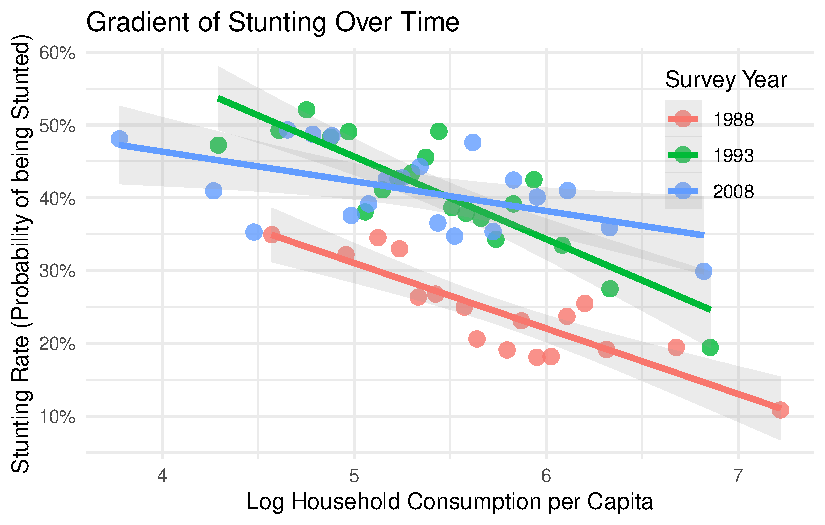
\includegraphics[keepaspectratio]{hw2_trimmed_files/figure-pdf/fig-over_time-1.pdf}}

}

}

\end{figure}%

 
\begin{table}[ht]
\begin{centerbox}
\begin{threeparttable}
\captionsetup{justification=centering,singlelinecheck=off}
\caption{Heterogeneous Effects of Consumption on Stunting Rates by Consumption Tertile}
 \label{tbl-stunting_by_income}\setlength{\tabcolsep}{0pt}
\begin{tabular}{l l l l l}


\hhline{>{\huxb{0, 0, 0}{0.8}}->{\huxb{0, 0, 0}{0.8}}->{\huxb{0, 0, 0}{0.8}}->{\huxb{0, 0, 0}{0.8}}->{\huxb{0, 0, 0}{0.8}}-}
\arrayrulecolor{black}

\multicolumn{1}{!{\huxvb{0, 0, 0}{0}}c!{\huxvb{0, 0, 0}{0}}}{\huxtpad{1.5pt + 1em}\centering \hspace{1.5pt}  \hspace{1.5pt}\huxbpad{1.5pt}} &
\multicolumn{1}{c!{\huxvb{0, 0, 0}{0}}}{\huxtpad{1.5pt + 1em}\centering \hspace{1.5pt} General (All) \hspace{1.5pt}\huxbpad{1.5pt}} &
\multicolumn{1}{c!{\huxvb{0, 0, 0}{0}}}{\huxtpad{1.5pt + 1em}\centering \hspace{1.5pt} Low Cons (T1) \hspace{1.5pt}\huxbpad{1.5pt}} &
\multicolumn{1}{c!{\huxvb{0, 0, 0}{0}}}{\huxtpad{1.5pt + 1em}\centering \hspace{1.5pt} Medium Cons (T2) \hspace{1.5pt}\huxbpad{1.5pt}} &
\multicolumn{1}{c!{\huxvb{0, 0, 0}{0}}}{\huxtpad{1.5pt + 1em}\centering \hspace{1.5pt} High Cons (T3) \hspace{1.5pt}\huxbpad{1.5pt}} \tabularnewline[-0.5pt]


\hhline{>{\huxb{255, 255, 255}{0.4}}->{\huxb{0, 0, 0}{0.4}}->{\huxb{0, 0, 0}{0.4}}->{\huxb{0, 0, 0}{0.4}}->{\huxb{0, 0, 0}{0.4}}-}
\arrayrulecolor{black}

\multicolumn{1}{!{\huxvb{0, 0, 0}{0}}l!{\huxvb{0, 0, 0}{0}}}{\huxtpad{1.5pt + 1em}\raggedright \hspace{1.5pt} Average Stunting Rate (1988) \hspace{1.5pt}\huxbpad{1.5pt}} &
\multicolumn{1}{r!{\huxvb{0, 0, 0}{0}}}{\huxtpad{1.5pt + 1em}\raggedleft \hspace{1.5pt} 0.371 *** \hspace{1.5pt}\huxbpad{1.5pt}} &
\multicolumn{1}{r!{\huxvb{0, 0, 0}{0}}}{\huxtpad{1.5pt + 1em}\raggedleft \hspace{1.5pt} 0.421 *** \hspace{1.5pt}\huxbpad{1.5pt}} &
\multicolumn{1}{r!{\huxvb{0, 0, 0}{0}}}{\huxtpad{1.5pt + 1em}\raggedleft \hspace{1.5pt} 0.393 *** \hspace{1.5pt}\huxbpad{1.5pt}} &
\multicolumn{1}{r!{\huxvb{0, 0, 0}{0}}}{\huxtpad{1.5pt + 1em}\raggedleft \hspace{1.5pt} 0.333 *** \hspace{1.5pt}\huxbpad{1.5pt}} \tabularnewline[-0.5pt]


\hhline{}
\arrayrulecolor{black}

\multicolumn{1}{!{\huxvb{0, 0, 0}{0}}l!{\huxvb{0, 0, 0}{0}}}{\huxtpad{1.5pt + 1em}\raggedright \hspace{1.5pt}  \hspace{1.5pt}\huxbpad{1.5pt}} &
\multicolumn{1}{r!{\huxvb{0, 0, 0}{0}}}{\huxtpad{1.5pt + 1em}\raggedleft \hspace{1.5pt} (0.021) \hspace{1.5pt}\huxbpad{1.5pt}} &
\multicolumn{1}{r!{\huxvb{0, 0, 0}{0}}}{\huxtpad{1.5pt + 1em}\raggedleft \hspace{1.5pt} (0.063) \hspace{1.5pt}\huxbpad{1.5pt}} &
\multicolumn{1}{r!{\huxvb{0, 0, 0}{0}}}{\huxtpad{1.5pt + 1em}\raggedleft \hspace{1.5pt} (0.036) \hspace{1.5pt}\huxbpad{1.5pt}} &
\multicolumn{1}{r!{\huxvb{0, 0, 0}{0}}}{\huxtpad{1.5pt + 1em}\raggedleft \hspace{1.5pt} (0.039) \hspace{1.5pt}\huxbpad{1.5pt}} \tabularnewline[-0.5pt]


\hhline{}
\arrayrulecolor{black}

\multicolumn{1}{!{\huxvb{0, 0, 0}{0}}l!{\huxvb{0, 0, 0}{0}}}{\huxtpad{1.5pt + 1em}\raggedright \hspace{1.5pt} Log Consumption (Centered) \hspace{1.5pt}\huxbpad{1.5pt}} &
\multicolumn{1}{r!{\huxvb{0, 0, 0}{0}}}{\huxtpad{1.5pt + 1em}\raggedleft \hspace{1.5pt} -0.074 *** \hspace{1.5pt}\huxbpad{1.5pt}} &
\multicolumn{1}{r!{\huxvb{0, 0, 0}{0}}}{\huxtpad{1.5pt + 1em}\raggedleft \hspace{1.5pt} 0.026 \hspace{1.5pt}\huxbpad{1.5pt}} &
\multicolumn{1}{r!{\huxvb{0, 0, 0}{0}}}{\huxtpad{1.5pt + 1em}\raggedleft \hspace{1.5pt} -0.136 \hspace{1.5pt}\huxbpad{1.5pt}} &
\multicolumn{1}{r!{\huxvb{0, 0, 0}{0}}}{\huxtpad{1.5pt + 1em}\raggedleft \hspace{1.5pt} -0.009 \hspace{1.5pt}\huxbpad{1.5pt}} \tabularnewline[-0.5pt]


\hhline{}
\arrayrulecolor{black}

\multicolumn{1}{!{\huxvb{0, 0, 0}{0}}l!{\huxvb{0, 0, 0}{0}}}{\huxtpad{1.5pt + 1em}\raggedright \hspace{1.5pt}  \hspace{1.5pt}\huxbpad{1.5pt}} &
\multicolumn{1}{r!{\huxvb{0, 0, 0}{0}}}{\huxtpad{1.5pt + 1em}\raggedleft \hspace{1.5pt} (0.014) \hspace{1.5pt}\huxbpad{1.5pt}} &
\multicolumn{1}{r!{\huxvb{0, 0, 0}{0}}}{\huxtpad{1.5pt + 1em}\raggedleft \hspace{1.5pt} (0.083) \hspace{1.5pt}\huxbpad{1.5pt}} &
\multicolumn{1}{r!{\huxvb{0, 0, 0}{0}}}{\huxtpad{1.5pt + 1em}\raggedleft \hspace{1.5pt} (0.101) \hspace{1.5pt}\huxbpad{1.5pt}} &
\multicolumn{1}{r!{\huxvb{0, 0, 0}{0}}}{\huxtpad{1.5pt + 1em}\raggedleft \hspace{1.5pt} (0.027) \hspace{1.5pt}\huxbpad{1.5pt}} \tabularnewline[-0.5pt]


\hhline{}
\arrayrulecolor{black}

\multicolumn{1}{!{\huxvb{0, 0, 0}{0}}l!{\huxvb{0, 0, 0}{0}}}{\huxtpad{1.5pt + 1em}\raggedright \hspace{1.5pt} Year 1993 Shift \hspace{1.5pt}\huxbpad{1.5pt}} &
\multicolumn{1}{r!{\huxvb{0, 0, 0}{0}}}{\huxtpad{1.5pt + 1em}\raggedleft \hspace{1.5pt} 0.138 *** \hspace{1.5pt}\huxbpad{1.5pt}} &
\multicolumn{1}{r!{\huxvb{0, 0, 0}{0}}}{\huxtpad{1.5pt + 1em}\raggedleft \hspace{1.5pt} 0.031 \hspace{1.5pt}\huxbpad{1.5pt}} &
\multicolumn{1}{r!{\huxvb{0, 0, 0}{0}}}{\huxtpad{1.5pt + 1em}\raggedleft \hspace{1.5pt} 0.156 *** \hspace{1.5pt}\huxbpad{1.5pt}} &
\multicolumn{1}{r!{\huxvb{0, 0, 0}{0}}}{\huxtpad{1.5pt + 1em}\raggedleft \hspace{1.5pt} 0.218 *** \hspace{1.5pt}\huxbpad{1.5pt}} \tabularnewline[-0.5pt]


\hhline{}
\arrayrulecolor{black}

\multicolumn{1}{!{\huxvb{0, 0, 0}{0}}l!{\huxvb{0, 0, 0}{0}}}{\huxtpad{1.5pt + 1em}\raggedright \hspace{1.5pt}  \hspace{1.5pt}\huxbpad{1.5pt}} &
\multicolumn{1}{r!{\huxvb{0, 0, 0}{0}}}{\huxtpad{1.5pt + 1em}\raggedleft \hspace{1.5pt} (0.012) \hspace{1.5pt}\huxbpad{1.5pt}} &
\multicolumn{1}{r!{\huxvb{0, 0, 0}{0}}}{\huxtpad{1.5pt + 1em}\raggedleft \hspace{1.5pt} (0.062) \hspace{1.5pt}\huxbpad{1.5pt}} &
\multicolumn{1}{r!{\huxvb{0, 0, 0}{0}}}{\huxtpad{1.5pt + 1em}\raggedleft \hspace{1.5pt} (0.019) \hspace{1.5pt}\huxbpad{1.5pt}} &
\multicolumn{1}{r!{\huxvb{0, 0, 0}{0}}}{\huxtpad{1.5pt + 1em}\raggedleft \hspace{1.5pt} (0.034) \hspace{1.5pt}\huxbpad{1.5pt}} \tabularnewline[-0.5pt]


\hhline{}
\arrayrulecolor{black}

\multicolumn{1}{!{\huxvb{0, 0, 0}{0}}l!{\huxvb{0, 0, 0}{0}}}{\huxtpad{1.5pt + 1em}\raggedright \hspace{1.5pt} Year 2008 Shift \hspace{1.5pt}\huxbpad{1.5pt}} &
\multicolumn{1}{r!{\huxvb{0, 0, 0}{0}}}{\huxtpad{1.5pt + 1em}\raggedleft \hspace{1.5pt} 0.150 *** \hspace{1.5pt}\huxbpad{1.5pt}} &
\multicolumn{1}{r!{\huxvb{0, 0, 0}{0}}}{\huxtpad{1.5pt + 1em}\raggedleft \hspace{1.5pt} 0.061 \hspace{1.5pt}\huxbpad{1.5pt}} &
\multicolumn{1}{r!{\huxvb{0, 0, 0}{0}}}{\huxtpad{1.5pt + 1em}\raggedleft \hspace{1.5pt} 0.158 *** \hspace{1.5pt}\huxbpad{1.5pt}} &
\multicolumn{1}{r!{\huxvb{0, 0, 0}{0}}}{\huxtpad{1.5pt + 1em}\raggedleft \hspace{1.5pt} 0.257 *** \hspace{1.5pt}\huxbpad{1.5pt}} \tabularnewline[-0.5pt]


\hhline{}
\arrayrulecolor{black}

\multicolumn{1}{!{\huxvb{0, 0, 0}{0}}l!{\huxvb{0, 0, 0}{0}}}{\huxtpad{1.5pt + 1em}\raggedright \hspace{1.5pt}  \hspace{1.5pt}\huxbpad{1.5pt}} &
\multicolumn{1}{r!{\huxvb{0, 0, 0}{0}}}{\huxtpad{1.5pt + 1em}\raggedleft \hspace{1.5pt} (0.013) \hspace{1.5pt}\huxbpad{1.5pt}} &
\multicolumn{1}{r!{\huxvb{0, 0, 0}{0}}}{\huxtpad{1.5pt + 1em}\raggedleft \hspace{1.5pt} (0.062) \hspace{1.5pt}\huxbpad{1.5pt}} &
\multicolumn{1}{r!{\huxvb{0, 0, 0}{0}}}{\huxtpad{1.5pt + 1em}\raggedleft \hspace{1.5pt} (0.023) \hspace{1.5pt}\huxbpad{1.5pt}} &
\multicolumn{1}{r!{\huxvb{0, 0, 0}{0}}}{\huxtpad{1.5pt + 1em}\raggedleft \hspace{1.5pt} (0.038) \hspace{1.5pt}\huxbpad{1.5pt}} \tabularnewline[-0.5pt]


\hhline{}
\arrayrulecolor{black}

\multicolumn{1}{!{\huxvb{0, 0, 0}{0}}l!{\huxvb{0, 0, 0}{0}}}{\huxtpad{1.5pt + 1em}\raggedright \hspace{1.5pt} Cons. Effect Diff (1993) \hspace{1.5pt}\huxbpad{1.5pt}} &
\multicolumn{1}{r!{\huxvb{0, 0, 0}{0}}}{\huxtpad{1.5pt + 1em}\raggedleft \hspace{1.5pt} -0.023 \hspace{1.5pt}\huxbpad{1.5pt}} &
\multicolumn{1}{r!{\huxvb{0, 0, 0}{0}}}{\huxtpad{1.5pt + 1em}\raggedleft \hspace{1.5pt} -0.124 \hspace{1.5pt}\huxbpad{1.5pt}} &
\multicolumn{1}{r!{\huxvb{0, 0, 0}{0}}}{\huxtpad{1.5pt + 1em}\raggedleft \hspace{1.5pt} -0.047 \hspace{1.5pt}\huxbpad{1.5pt}} &
\multicolumn{1}{r!{\huxvb{0, 0, 0}{0}}}{\huxtpad{1.5pt + 1em}\raggedleft \hspace{1.5pt} -0.121 *** \hspace{1.5pt}\huxbpad{1.5pt}} \tabularnewline[-0.5pt]


\hhline{}
\arrayrulecolor{black}

\multicolumn{1}{!{\huxvb{0, 0, 0}{0}}l!{\huxvb{0, 0, 0}{0}}}{\huxtpad{1.5pt + 1em}\raggedright \hspace{1.5pt}  \hspace{1.5pt}\huxbpad{1.5pt}} &
\multicolumn{1}{r!{\huxvb{0, 0, 0}{0}}}{\huxtpad{1.5pt + 1em}\raggedleft \hspace{1.5pt} (0.018) \hspace{1.5pt}\huxbpad{1.5pt}} &
\multicolumn{1}{r!{\huxvb{0, 0, 0}{0}}}{\huxtpad{1.5pt + 1em}\raggedleft \hspace{1.5pt} (0.092) \hspace{1.5pt}\huxbpad{1.5pt}} &
\multicolumn{1}{r!{\huxvb{0, 0, 0}{0}}}{\huxtpad{1.5pt + 1em}\raggedleft \hspace{1.5pt} (0.126) \hspace{1.5pt}\huxbpad{1.5pt}} &
\multicolumn{1}{r!{\huxvb{0, 0, 0}{0}}}{\huxtpad{1.5pt + 1em}\raggedleft \hspace{1.5pt} (0.041) \hspace{1.5pt}\huxbpad{1.5pt}} \tabularnewline[-0.5pt]


\hhline{}
\arrayrulecolor{black}

\multicolumn{1}{!{\huxvb{0, 0, 0}{0}}l!{\huxvb{0, 0, 0}{0}}}{\huxtpad{1.5pt + 1em}\raggedright \hspace{1.5pt} Cons. Effect Diff (2008) \hspace{1.5pt}\huxbpad{1.5pt}} &
\multicolumn{1}{r!{\huxvb{0, 0, 0}{0}}}{\huxtpad{1.5pt + 1em}\raggedleft \hspace{1.5pt} 0.047 *** \hspace{1.5pt}\huxbpad{1.5pt}} &
\multicolumn{1}{r!{\huxvb{0, 0, 0}{0}}}{\huxtpad{1.5pt + 1em}\raggedleft \hspace{1.5pt} -0.032 \hspace{1.5pt}\huxbpad{1.5pt}} &
\multicolumn{1}{r!{\huxvb{0, 0, 0}{0}}}{\huxtpad{1.5pt + 1em}\raggedleft \hspace{1.5pt} 0.020 \hspace{1.5pt}\huxbpad{1.5pt}} &
\multicolumn{1}{r!{\huxvb{0, 0, 0}{0}}}{\huxtpad{1.5pt + 1em}\raggedleft \hspace{1.5pt} -0.081 * \hspace{1.5pt}\huxbpad{1.5pt}} \tabularnewline[-0.5pt]


\hhline{}
\arrayrulecolor{black}

\multicolumn{1}{!{\huxvb{0, 0, 0}{0}}l!{\huxvb{0, 0, 0}{0}}}{\huxtpad{1.5pt + 1em}\raggedright \hspace{1.5pt}  \hspace{1.5pt}\huxbpad{1.5pt}} &
\multicolumn{1}{r!{\huxvb{0, 0, 0}{0}}}{\huxtpad{1.5pt + 1em}\raggedleft \hspace{1.5pt} (0.018) \hspace{1.5pt}\huxbpad{1.5pt}} &
\multicolumn{1}{r!{\huxvb{0, 0, 0}{0}}}{\huxtpad{1.5pt + 1em}\raggedleft \hspace{1.5pt} (0.088) \hspace{1.5pt}\huxbpad{1.5pt}} &
\multicolumn{1}{r!{\huxvb{0, 0, 0}{0}}}{\huxtpad{1.5pt + 1em}\raggedleft \hspace{1.5pt} (0.141) \hspace{1.5pt}\huxbpad{1.5pt}} &
\multicolumn{1}{r!{\huxvb{0, 0, 0}{0}}}{\huxtpad{1.5pt + 1em}\raggedleft \hspace{1.5pt} (0.045) \hspace{1.5pt}\huxbpad{1.5pt}} \tabularnewline[-0.5pt]


\hhline{>{\huxb{255, 255, 255}{0.4}}->{\huxb{0, 0, 0}{0.4}}->{\huxb{0, 0, 0}{0.4}}->{\huxb{0, 0, 0}{0.4}}->{\huxb{0, 0, 0}{0.4}}-}
\arrayrulecolor{black}

\multicolumn{1}{!{\huxvb{0, 0, 0}{0}}l!{\huxvb{0, 0, 0}{0}}}{\huxtpad{1.5pt + 1em}\raggedright \hspace{1.5pt} Controls \hspace{1.5pt}\huxbpad{1.5pt}} &
\multicolumn{1}{r!{\huxvb{0, 0, 0}{0}}}{\huxtpad{1.5pt + 1em}\raggedleft \hspace{1.5pt} Yes \hspace{1.5pt}\huxbpad{1.5pt}} &
\multicolumn{1}{r!{\huxvb{0, 0, 0}{0}}}{\huxtpad{1.5pt + 1em}\raggedleft \hspace{1.5pt} Yes \hspace{1.5pt}\huxbpad{1.5pt}} &
\multicolumn{1}{r!{\huxvb{0, 0, 0}{0}}}{\huxtpad{1.5pt + 1em}\raggedleft \hspace{1.5pt} Yes \hspace{1.5pt}\huxbpad{1.5pt}} &
\multicolumn{1}{r!{\huxvb{0, 0, 0}{0}}}{\huxtpad{1.5pt + 1em}\raggedleft \hspace{1.5pt} Yes \hspace{1.5pt}\huxbpad{1.5pt}} \tabularnewline[-0.5pt]


\hhline{>{\huxb{255, 255, 255}{0.4}}->{\huxb{0, 0, 0}{0.4}}->{\huxb{0, 0, 0}{0.4}}->{\huxb{0, 0, 0}{0.4}}->{\huxb{0, 0, 0}{0.4}}-}
\arrayrulecolor{black}

\multicolumn{1}{!{\huxvb{0, 0, 0}{0}}l!{\huxvb{0, 0, 0}{0}}}{\huxtpad{1.5pt + 1em}\raggedright \hspace{1.5pt} Outliers Excluded \hspace{1.5pt}\huxbpad{1.5pt}} &
\multicolumn{1}{r!{\huxvb{0, 0, 0}{0}}}{\huxtpad{1.5pt + 1em}\raggedleft \hspace{1.5pt} Yes \hspace{1.5pt}\huxbpad{1.5pt}} &
\multicolumn{1}{r!{\huxvb{0, 0, 0}{0}}}{\huxtpad{1.5pt + 1em}\raggedleft \hspace{1.5pt} Yes \hspace{1.5pt}\huxbpad{1.5pt}} &
\multicolumn{1}{r!{\huxvb{0, 0, 0}{0}}}{\huxtpad{1.5pt + 1em}\raggedleft \hspace{1.5pt} Yes \hspace{1.5pt}\huxbpad{1.5pt}} &
\multicolumn{1}{r!{\huxvb{0, 0, 0}{0}}}{\huxtpad{1.5pt + 1em}\raggedleft \hspace{1.5pt} Yes \hspace{1.5pt}\huxbpad{1.5pt}} \tabularnewline[-0.5pt]


\hhline{>{\huxb{255, 255, 255}{0.4}}->{\huxb{0, 0, 0}{0.4}}->{\huxb{0, 0, 0}{0.4}}->{\huxb{0, 0, 0}{0.4}}->{\huxb{0, 0, 0}{0.4}}-}
\arrayrulecolor{black}

\multicolumn{1}{!{\huxvb{0, 0, 0}{0}}l!{\huxvb{0, 0, 0}{0}}}{\huxtpad{1.5pt + 1em}\raggedright \hspace{1.5pt} N \hspace{1.5pt}\huxbpad{1.5pt}} &
\multicolumn{1}{r!{\huxvb{0, 0, 0}{0}}}{\huxtpad{1.5pt + 1em}\raggedleft \hspace{1.5pt} 10897 \hspace{1.5pt}\huxbpad{1.5pt}} &
\multicolumn{1}{r!{\huxvb{0, 0, 0}{0}}}{\huxtpad{1.5pt + 1em}\raggedleft \hspace{1.5pt} 3634 \hspace{1.5pt}\huxbpad{1.5pt}} &
\multicolumn{1}{r!{\huxvb{0, 0, 0}{0}}}{\huxtpad{1.5pt + 1em}\raggedleft \hspace{1.5pt} 3631 \hspace{1.5pt}\huxbpad{1.5pt}} &
\multicolumn{1}{r!{\huxvb{0, 0, 0}{0}}}{\huxtpad{1.5pt + 1em}\raggedleft \hspace{1.5pt} 3632 \hspace{1.5pt}\huxbpad{1.5pt}} \tabularnewline[-0.5pt]


\hhline{}
\arrayrulecolor{black}

\multicolumn{1}{!{\huxvb{0, 0, 0}{0}}l!{\huxvb{0, 0, 0}{0}}}{\huxtpad{1.5pt + 1em}\raggedright \hspace{1.5pt} R2 \hspace{1.5pt}\huxbpad{1.5pt}} &
\multicolumn{1}{r!{\huxvb{0, 0, 0}{0}}}{\huxtpad{1.5pt + 1em}\raggedleft \hspace{1.5pt} 0.043 \hspace{1.5pt}\huxbpad{1.5pt}} &
\multicolumn{1}{r!{\huxvb{0, 0, 0}{0}}}{\huxtpad{1.5pt + 1em}\raggedleft \hspace{1.5pt} 0.009 \hspace{1.5pt}\huxbpad{1.5pt}} &
\multicolumn{1}{r!{\huxvb{0, 0, 0}{0}}}{\huxtpad{1.5pt + 1em}\raggedleft \hspace{1.5pt} 0.032 \hspace{1.5pt}\huxbpad{1.5pt}} &
\multicolumn{1}{r!{\huxvb{0, 0, 0}{0}}}{\huxtpad{1.5pt + 1em}\raggedleft \hspace{1.5pt} 0.053 \hspace{1.5pt}\huxbpad{1.5pt}} \tabularnewline[-0.5pt]


\hhline{>{\huxb{0, 0, 0}{0.8}}->{\huxb{0, 0, 0}{0.8}}->{\huxb{0, 0, 0}{0.8}}->{\huxb{0, 0, 0}{0.8}}->{\huxb{0, 0, 0}{0.8}}-}
\arrayrulecolor{black}
\end{tabular}
\begin{tablenotes}[flushleft]
\item[] Significance: *** p $<$ 0.01; ** p $<$ 0.05; * p $<$ 0.1
\end{tablenotes}
\end{threeparttable}\par\end{centerbox}

\end{table}
 

\section{3 A meaningful table (6 pts)}\label{a-meaningful-table-6-pts}

In classical economics, the Tiebout model predicts that in the absence
of friction, individuals will ``vote with their feet'' and relocate to
countries offering the optimal bundle of public services, economic
opportunities, and living conditions. In reality, cross-border mobility
is heavily constrained by structural frictions, including relocation
costs, social capital networks, and national border regimes. In this
policy note, I evaluate the average share of foreign populations
(non-citizens) across OECD countries from 2013 to 2023, comparing
national baselines to understand how legal frameworks and integration
policies shape global demographic stocks.

Figure \ref{fig-migration} illustrates the OECD average share of foreign
population from 2013 to 2023, defined as usual residents residing in a
host country for at least twelve months without holding citizenship.
Following standard OECD and UN definitions, this metric captures
long-term foreign residents---including those on work visas, student
visas, and permanent residency permits, while strictly excluding
short-term tourists and temporary visitors. Across the OECD sample, this
non-citizen share grew from 5.5\% in 2013 to 7.2\% in 2023, reflecting
an increment in long-term international mobility despite persistent
institutional barriers. Confidence intervals for the OECD are shown in
the figure, but individual country-level confidence intervals are
omitted because they come from aggregated data.

Figure \ref{fig-migration} further demonstrates substantial
cross-country variance around this global baseline, which can be
evaluated across three distinct policy models:

\begin{enumerate}
\def\labelenumi{\arabic{enumi}.}
\tightlist
\item
  \textbf{Countries above the mean}: Germany maintains an high foreign
  population share of 15.8\% as of 2023. Historically, Germany has
  absorbed large-scale labor and humanitarian inflows, including
  post-WWII reconstruction labor, the 2015 Syrian refugee crisis, and
  displacement from the 2022 war in Ukraine. This high stock is
  sustained by active policy engineering, such as recent legislative
  reforms designed to lower administrative friction for skilled foreign
  workers.
\item
  \textbf{Countries below the mean}: Poland exhibits a deeply suppressed
  foreign population share of just 1.1\% in 2023. Unlike Western Europe,
  Poland maintained extreme demographic homogeneity throughout the
  post-WWII era and underwent a difficult post-communist economic
  transition that historically made it an exporter, rather than a
  destination, for labor. Furthermore, Polish immigration policy has
  traditionally favored temporary or seasonal labor migration from
  neighboring states over long-term structural integration.
\item
  \textbf{Countries near the mean}: The United States (8.4\%) and France
  (7.1\%) hover near the OECD baseline. Both nations maintain
  long-standing immigration traditions and strong international appeal
  for students and workers. However, their foreign national stocks
  remain moderate primarily due to robust naturalization pathways. As
  long-term residents acquire citizenship, they exit the ``foreign
  population'' metric, keeping non-citizen stocks stable despite
  continuous inbound migration.
\end{enumerate}

Evaluating these structural differences is vital for economic policy.
Nations with high foreign population stocks must focus on removing labor
market hurdles and enhancing civic integration, whereas countries with
suppressed foreign shares must streamline administrative visa processes
to remain competitive in attracting global talent.

\begin{figure}

\caption{\label{fig-migration}Stock of foreign population (non-citizens)
over time}

\centering{

\subcaption{\label{fig-migration}The dashed line represents the OECD
stock of foreign population (non-citizens), while the solid lines are
selected countries.}

\centering{

\pandocbounded{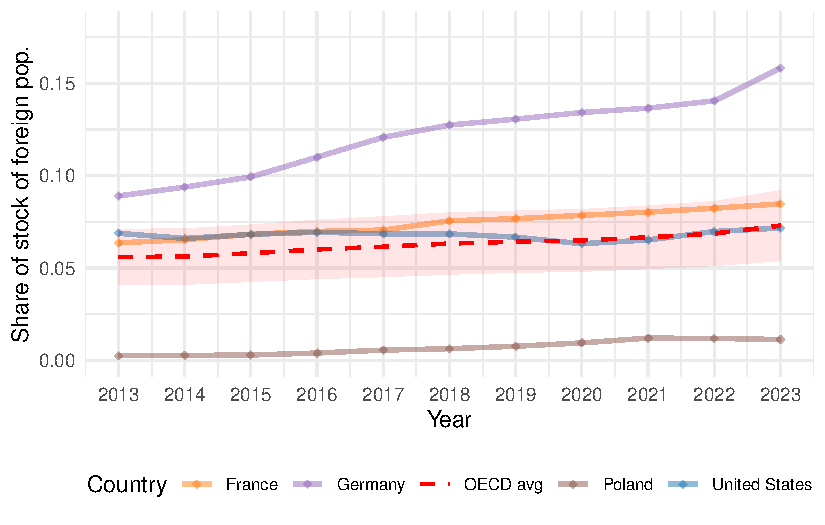
\includegraphics[keepaspectratio]{hw2_trimmed_files/figure-pdf/fig-migration-1.pdf}}

}

}

\end{figure}%

\section{Appendix R Script}\label{appendix-r-script}




\end{document}
